\subsubsection{\ystar\ cut optimisation}
\label{section:ystarCutOptimization}

%\todo[inline]{ Clean up formulae. }

In QCD, $t$-channel in 2-to-2 scattering is the dominant process. Thus the dijet production from the QCD is proportional to $\displaystyle{(1-\cos\theta^{*})^{-2}}$. However the distribution of $\cos\theta^{*}$ is supposed to be flat for signal, which means the \ystar\ of signal will peak at 0 while that of QCD background will minimize at 0.


The significance is defined as: 
\begin{equation}
\label{eq:signifcanceYstar} % uncomment if label used.
S  = \sqrt{\sum_{i}{2\left[ \left(S_{i}+B_{i} \right)\cdot \ln \left(1+\frac{S_{i}}{B_{i}}\right)-S_{i}\right]}}
\end{equation}
where $S_i$ ($B_i$) is the number of signal (background) events in bin $i$. 
The calculation of such significance only include the bins where signal samples have 95\% of the area under the distribution, not include the entire \mjj\ distribution.

For some signal samples where $S_i$ is small ($S_i << 10^{-5}$) thus the logarithm functions do not have
enough precision in equation \ref{eq:signifcanceYstar}. An approximation is introduced as follows:
\begin{equation}
%\label{eq:significanceYstarApprox}
S = \sqrt{\sum_{i}{2\sum_{n=1}^{6}{\frac{(-S_i)^{n+1}}{n \left(n+1 \right) B_i^n}}}}
\end{equation}
which is accurate up to 10 decimal places around $\frac{S_i}{B_i} = 10^{-5}$ and even more precise for smaller $\frac{S_i}{B_i}$.

%The significance of $H^\prime$ signal as a function 
%of the value of the \ystar\ is shown in Figure.~\ref{fig: hprime significance as a function of y* cut}. The peaks of significance in all tagging categories are around 0.6, therefore an optimal $y^{*}$ cut for the $H'$ search is set to
%$|\ystar| < 0.6$. The exact values of \ystar\ cut that correspond to the peak significance value for the $H^\prime$ signal at each mass point are shown in Table~\ref{tab:ystarhprime} with the ranges in \ystar\ cut around the peak that gives a significance $\geq$ 0.99.
%
%\begin{figure}[!htb]
%        \centering
%        \subfloat[Inclusive]{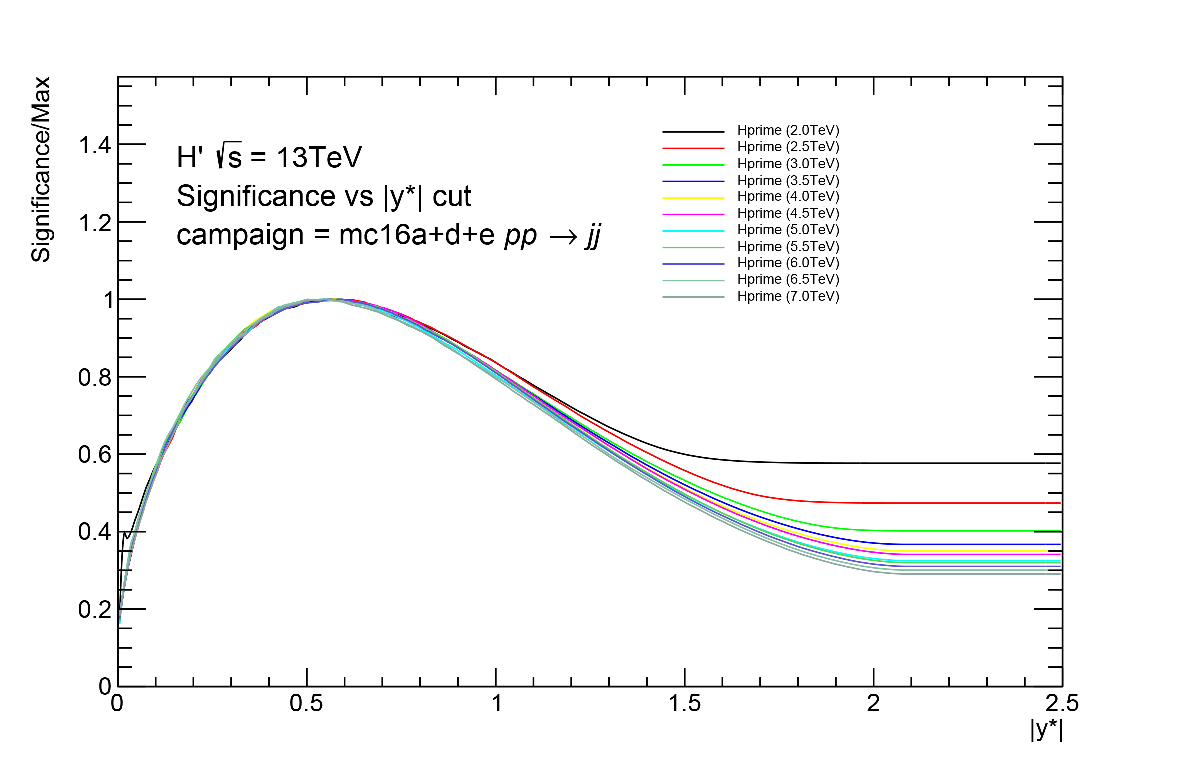
\includegraphics[width=0.45\columnwidth]{fig/yStarOptimization/New_Plots/Significance_Hprime_mc16a+d+e_jj.pdf}}
%        \subfloat[$\geq$1 g-tag]{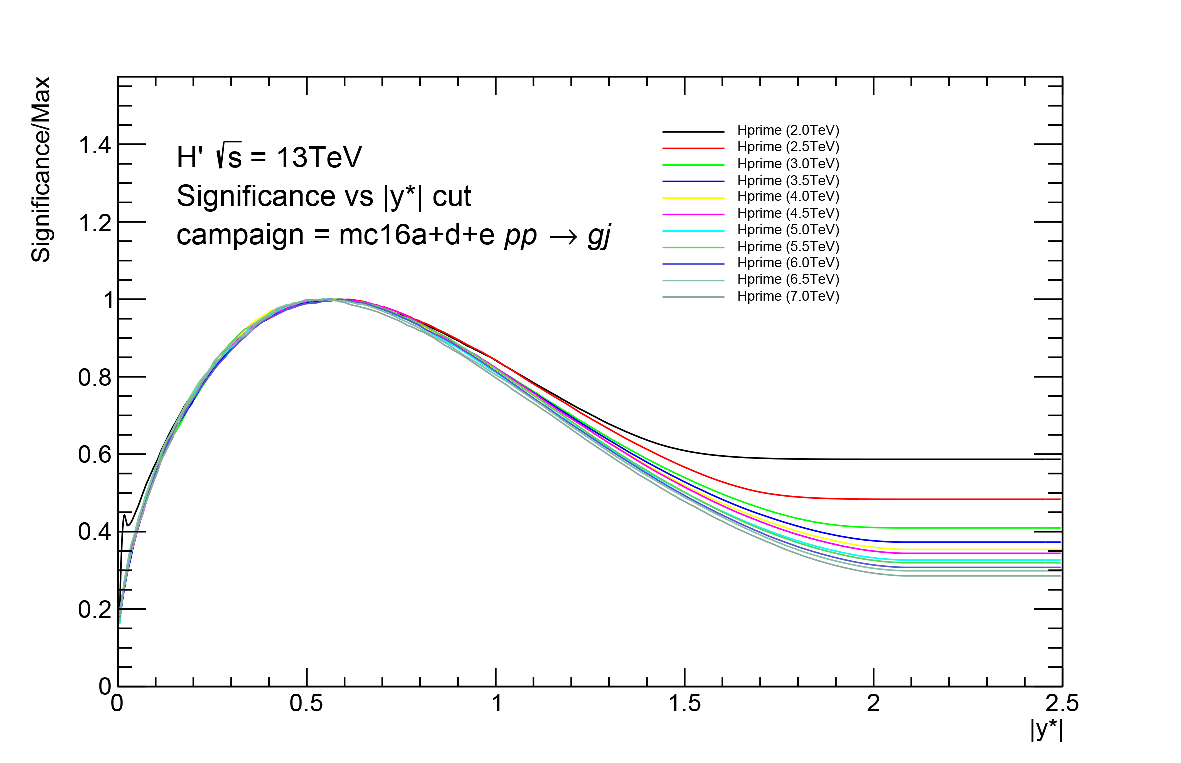
\includegraphics[width=0.45\columnwidth]{fig/yStarOptimization/New_Plots/Significance_Hprime_mc16a+d+e_gj.pdf}}\\
%        \subfloat[2 g-tag]{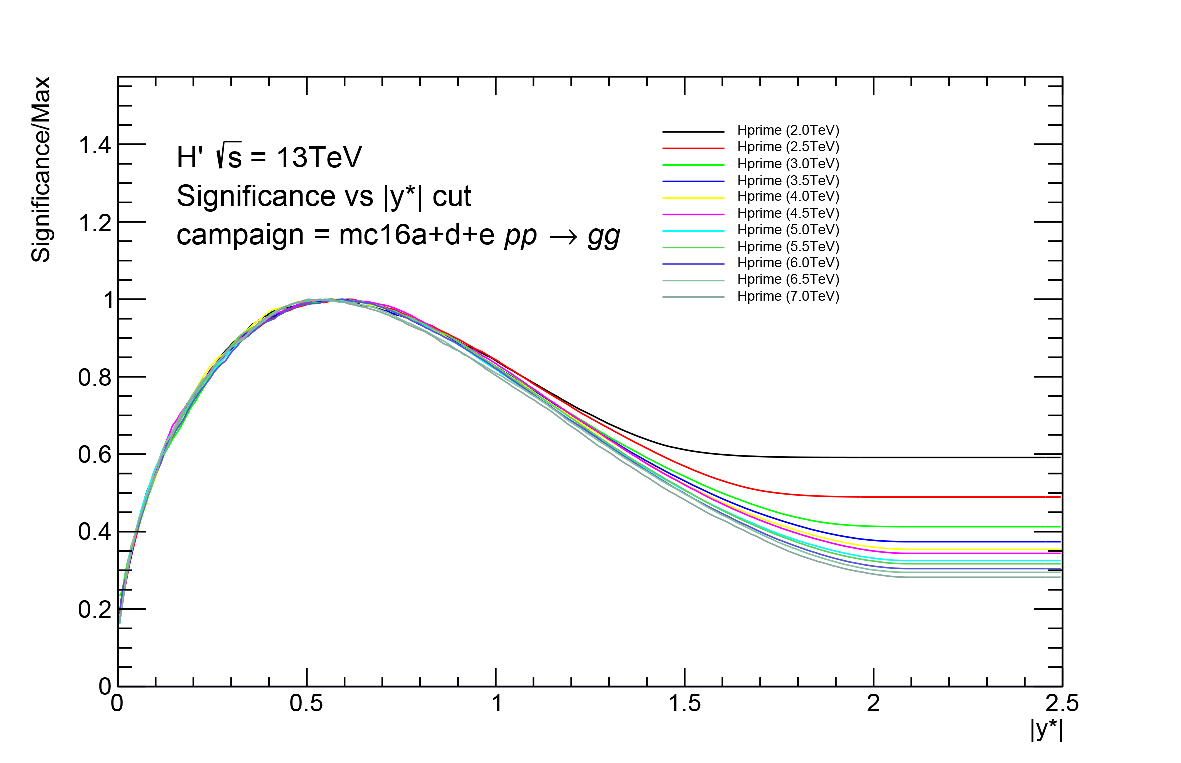
\includegraphics[width=0.45\columnwidth]{fig/yStarOptimization/New_Plots/Significance_Hprime_mc16a+d+e_gg.pdf}}
%        \caption{$H^\prime$ significance as a function \ystar\ cut in the case of (a) Inclusive, (b) $\geq$1 g-tag, (c) 2 g-tag.}
%        \label{fig: hprime significance as a function of y* cut}
%\end{figure}
% 
%
%\begin{table}[!htb]
%\begin{center}
%\begin{tabular}{ccccc}
%\toprule
%\multicolumn{1}{c}{$H^\prime$ Mass (TeV) } & \multicolumn{3}{c}{Optimal Selection} & \multicolumn{1}{c}{Peak Width} \\
%& \multicolumn{1}{c|}{Inclusive} & \multicolumn{1}{c|}{$\geq1$ $g$ tag} & \multicolumn{1}{c}{2 $g$ tag} \\
%\midrule
%2.0 & 0.57 & 0.57 & 0.57 & 0.50\text{--}0.65 \\
%2.5 & 0.58 & 0.59 & 0.62 & 0.50\text{--}0.67 \\
%3.0 & 0.59 & 0.59 & 0.59 & 0.50\text{--}0.66 \\
%3.5 & 0.56 & 0.56 & 0.60 & 0.49\text{--}0.65 \\
%4.0 & 0.58 & 0.58 & 0.58 & 0.47\text{--}0.65 \\
%4.5 & 0.55 & 0.57 & 0.57 & 0.35\text{--}0.68 \\
%5.0 & 0.55 & 0.56 & 0.57 & 0.47\text{--}0.66 \\
%5.5 & 0.55 & 0.55 & 0.57 & 0.46\text{--}0.66 \\
%6.0 & 0.60 & 0.60 & 0.60 & 0.52\text{--}0.66 \\
%6.5 & 0.55 & 0.55 & 0.54 & 0.47\text{--}0.64 \\
%7.0 & 0.56 & 0.56 & 0.51 & 0.35\text{--}0.61 \\
%\bottomrule
%\end{tabular}
%\end{center}
%\caption{$|y^*|$ selection leading to the maximum significance value calculated using Equation~\ref{eq:signifcanceYstar}.}\label{tab:ystarhprime}
%\end{table}

%For String signal, there is also a dependence on $\cos\theta^{*}$, leads the \ystar\ will peak at 0 too. Figure.~\ref{fig: string significance as a function of y* cut} shows the significance of String signal as a function of \ystar\ cut. The maximum significance in all tagging categories are around 0.8, therefore an optimal $y^{*}$ cut for the String search is set to $|\ystar| < 0.8$. The exact values of \ystar\ cut that correspond to the peak significance value for the String signal at each mass point are shown in Table.~\ref{tab:ystarstring} with the ranges in \ystar\ cut around the peak that gives a significance $\geq$ 0.99.
%
%\begin{figure}[!htb]
%        \centering
%        \subfloat[Inclusive]{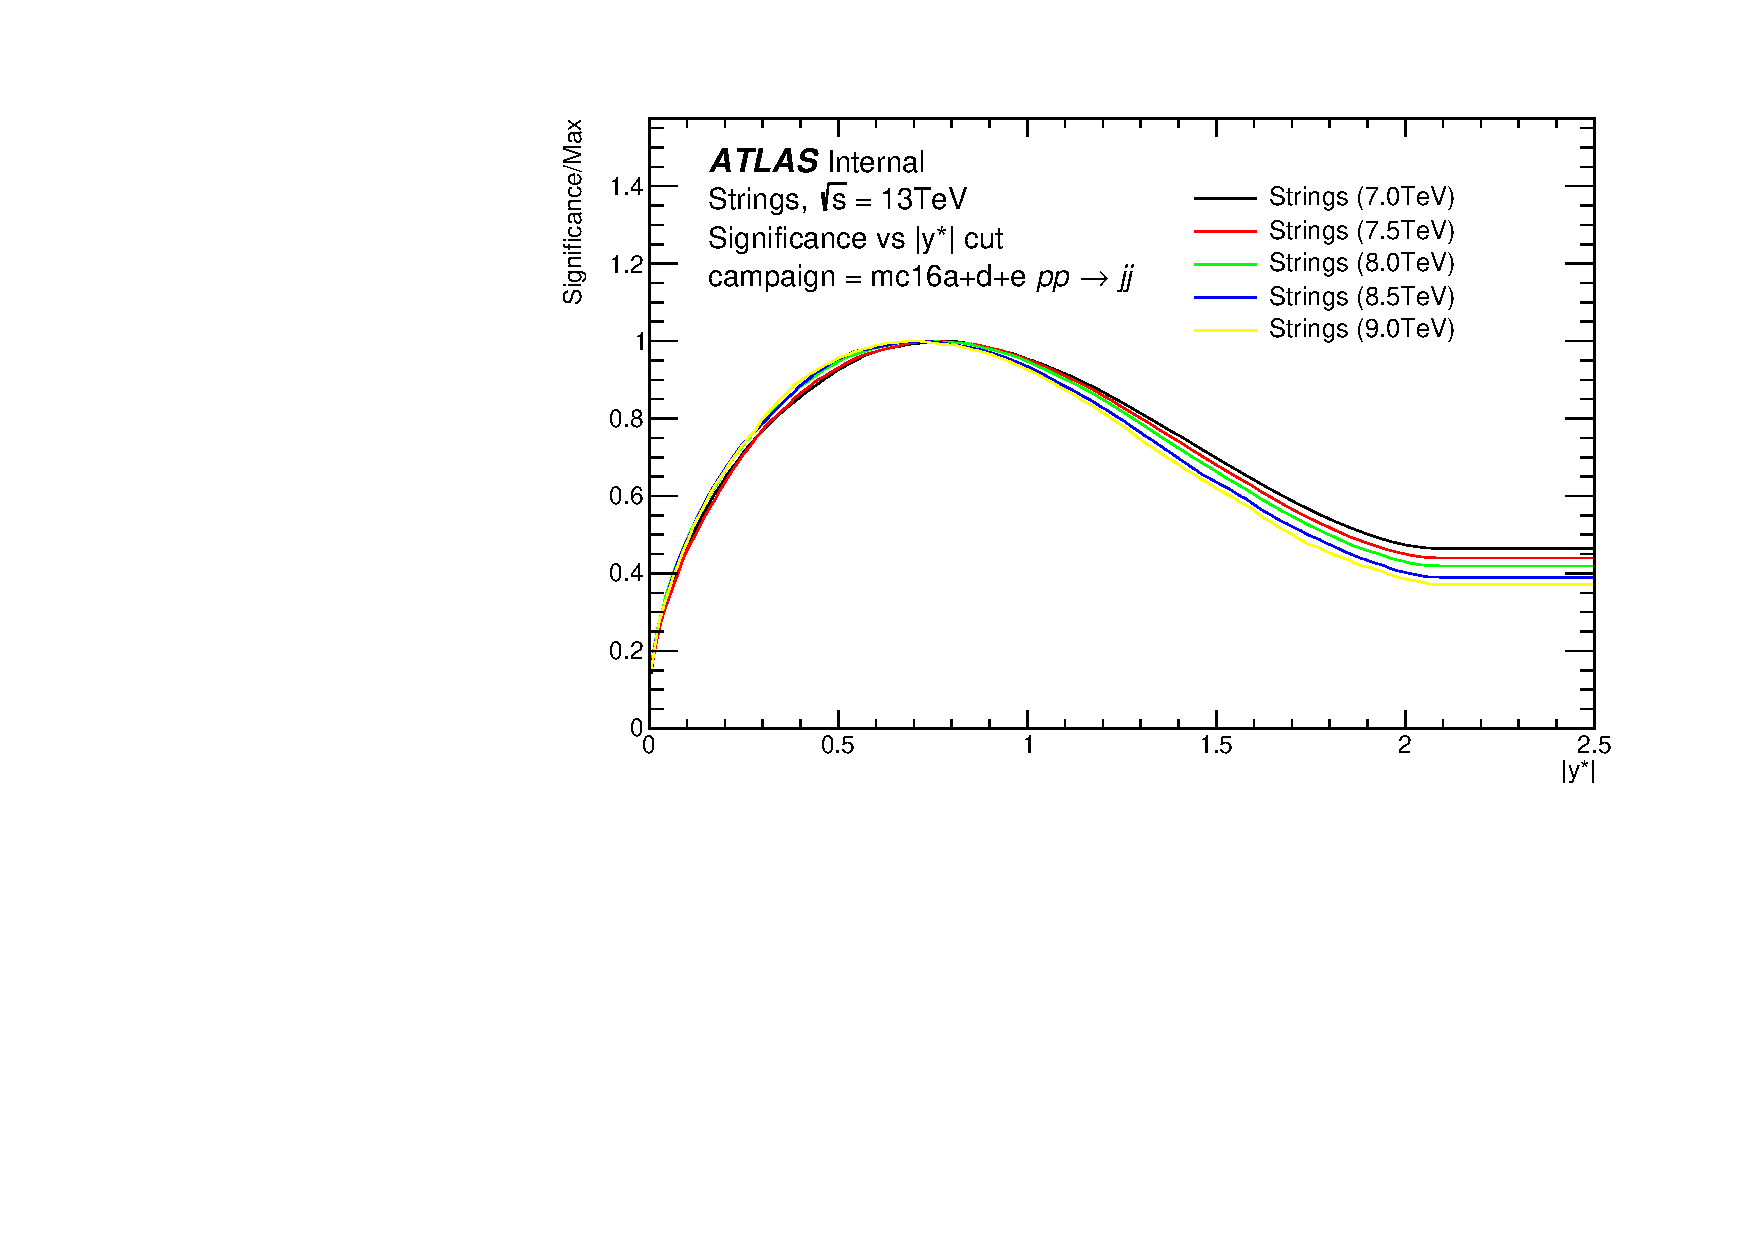
\includegraphics[width=0.45\columnwidth]{fig/yStarOptimization/New_Plots/Significance_Strings_mc16a+d+e_jj.pdf}}
%        \subfloat[$\geq$1 g-tag]{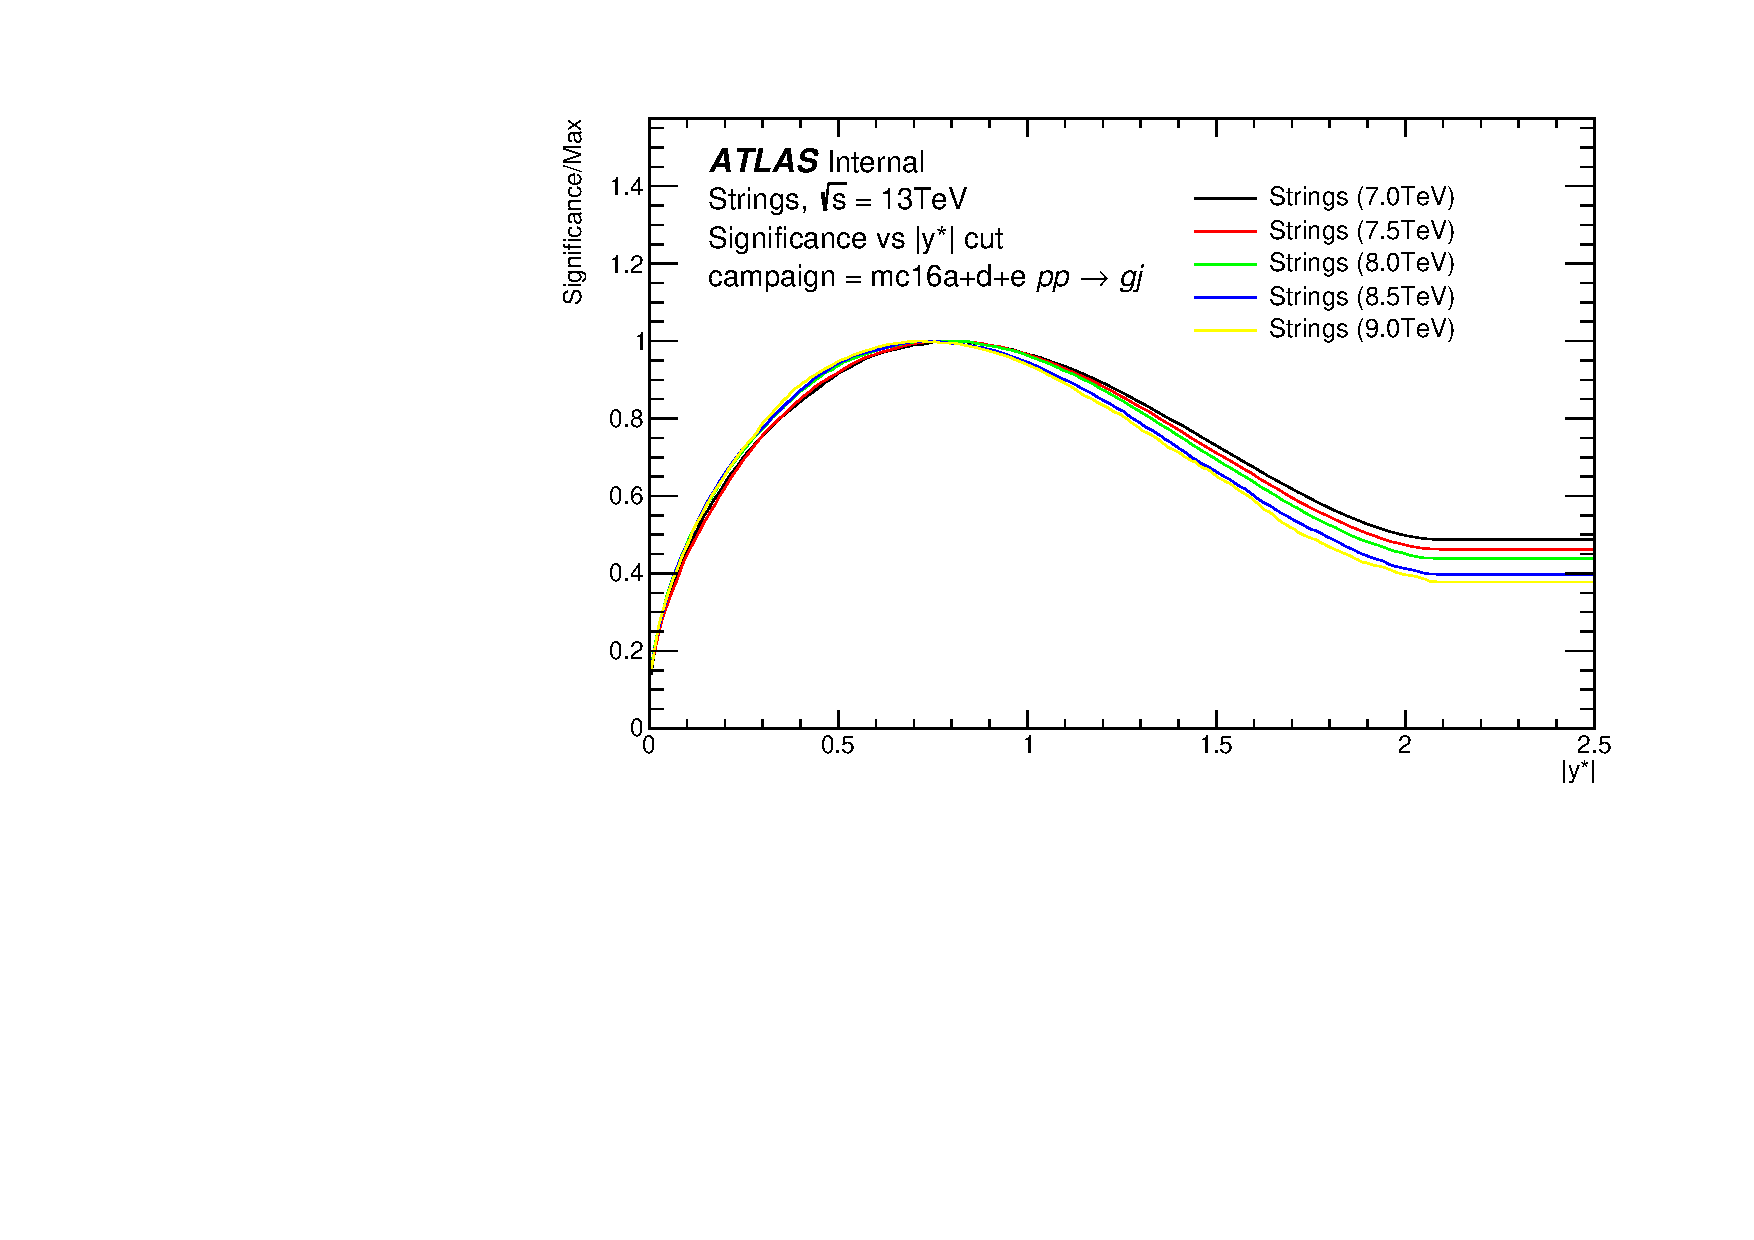
\includegraphics[width=0.45\columnwidth]{fig/yStarOptimization/New_Plots/Significance_Strings_mc16a+d+e_gj.pdf}}\\
%        \subfloat[2 g-tag]{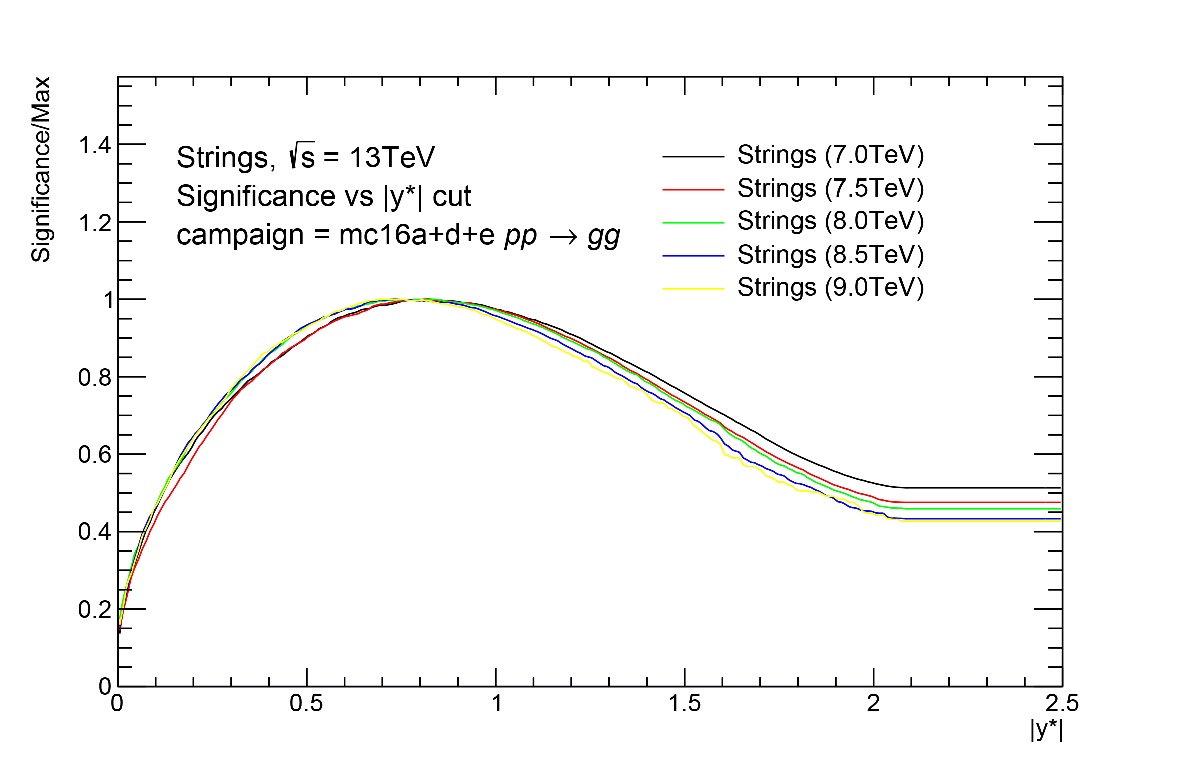
\includegraphics[width=0.45\columnwidth]{fig/yStarOptimization/New_Plots/Significance_Strings_mc16a+d+e_gg.pdf}}
%        \caption{String significance as a function \ystar\ cut in the case of (a) Inclusive, (b) $\geq$1 g-tag, (c) 2 g-tag.}
%        \label{fig: string significance as a function of y* cut}
%\end{figure}
%
%
%\begin{table}[!htb]
%\begin{center}
%\begin{tabular}{ccccc}
%\toprule
%\multicolumn{1}{c}{String Mass (TeV) } & \multicolumn{3}{c}{Optimal Selection} & \multicolumn{1}{c}{Peak Width} \\
%& \multicolumn{1}{c|}{Inclusive} & \multicolumn{1}{c|}{$\geq1$ $g$ tag} & \multicolumn{1}{c}{2 $g$ tag} \\
%\midrule
%7.0 & 0.78 & 0.82 & 0.81 & 0.70\text{--}0.91 \\
%7.5 & 0.77 & 0.77 & 0.83 & 0.68\text{--}0.91 \\
%8.0 & 0.72 & 0.76 & 0.84 & 0.66\text{--}0.90 \\
%8.5 & 0.74 & 0.74 & 0.74 & 0.65\text{--}0.85 \\
%9.0 & 0.71 & 0.71 & 0.71 & 0.62\text{--}0.84 \\
%\bottomrule
%\end{tabular}
%\end{center}
%\caption{$|y^*|$ selection leading to the maximum significance value calculated using Equation~\ref{eq:signifcanceYstar}.}\label{tab:ystarstring}
%\end{table}
%


Figure.~\ref{fig: graviton significance as a function of y* cut} shows the significance of Graviton signal as a function of \ystar\ cut. The significance peaks at about 0.6 to 0.8. Table~\ref{tab:ystargraviton} shows the \ystar\ cut corresponding to the peak significance value for Graviton at each mass point, and the range in \ystar\ cut around the peak that gives a significance $\geq$ 0.99
\begin{figure}[!htb]
        \centering
        \subfloat[Inclusive]{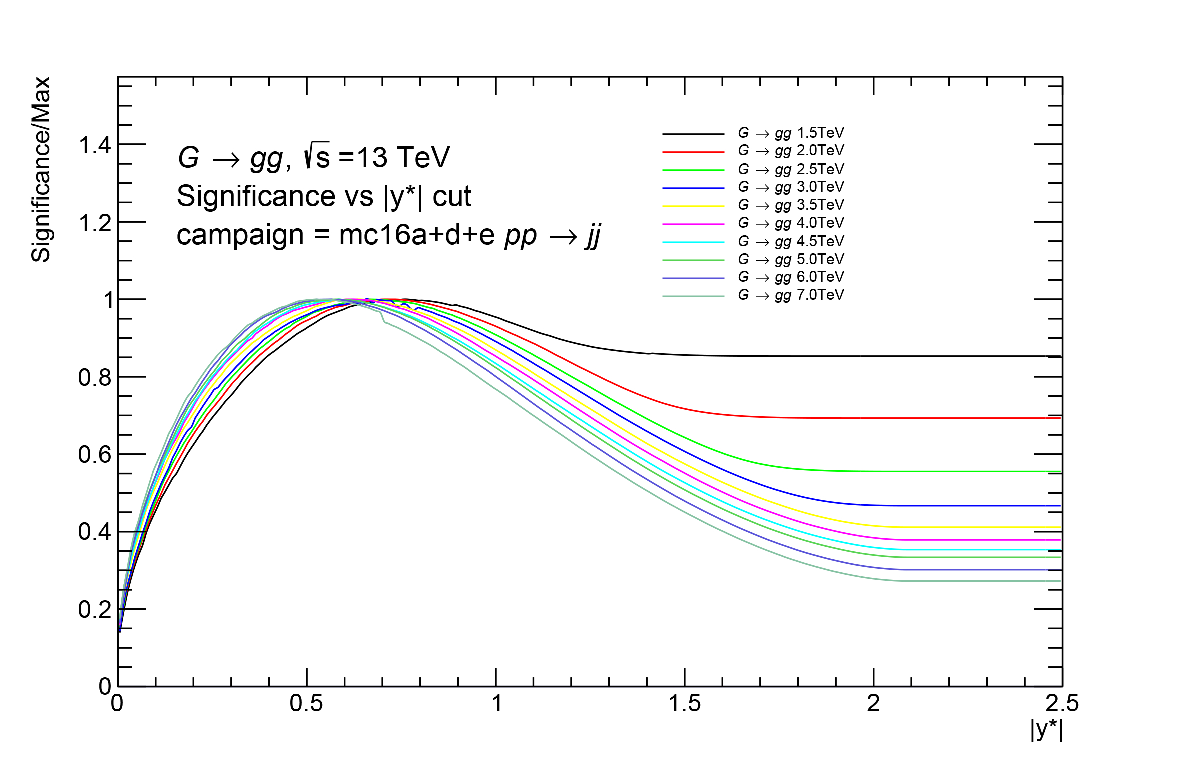
\includegraphics[width=0.45\columnwidth]{fig/yStarOptimization/New_Plots/Significance_Graviton_mc16a+d+e_jj.pdf}}
        \subfloat[$\geq$1 g-tag]{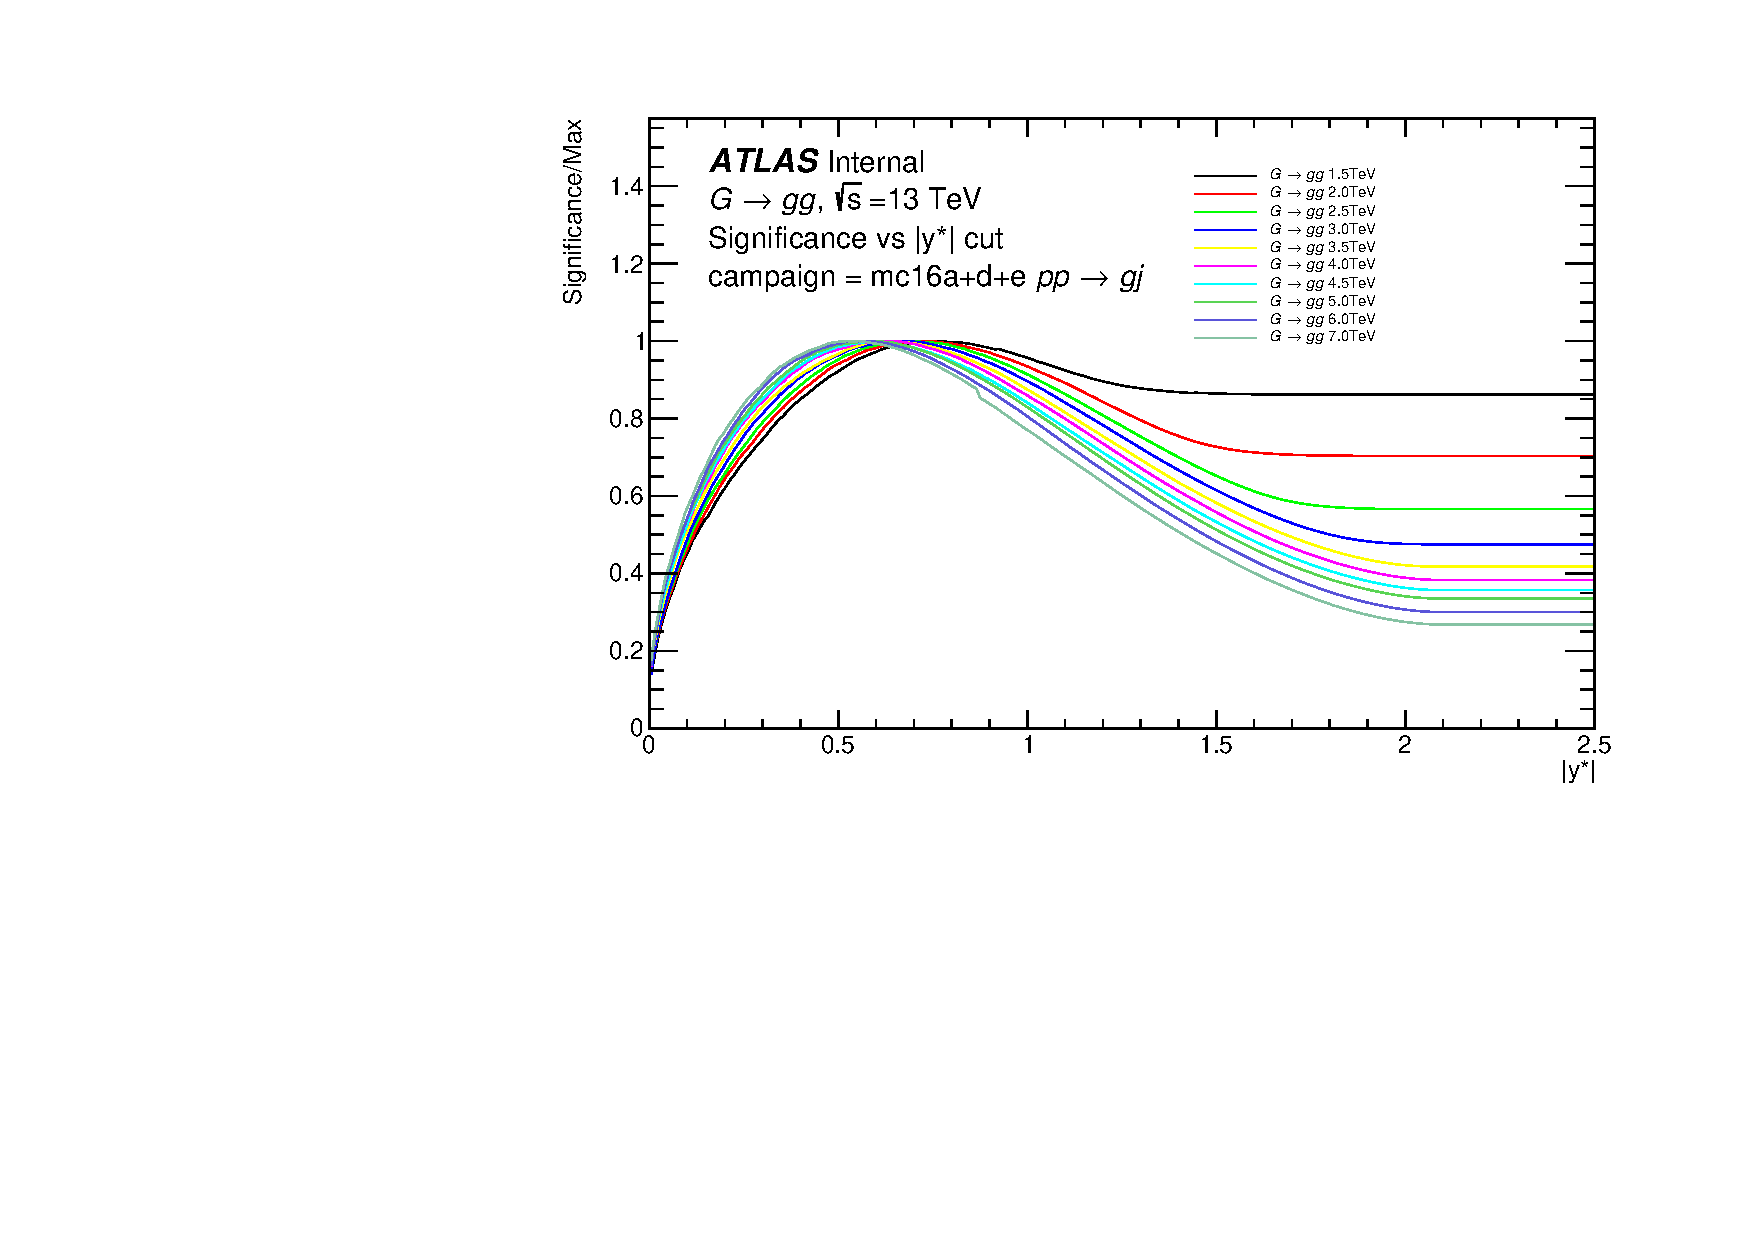
\includegraphics[width=0.45\columnwidth]{fig/yStarOptimization/New_Plots/Significance_Graviton_mc16a+d+e_gj.pdf}}\\
        \subfloat[2 g-tag]{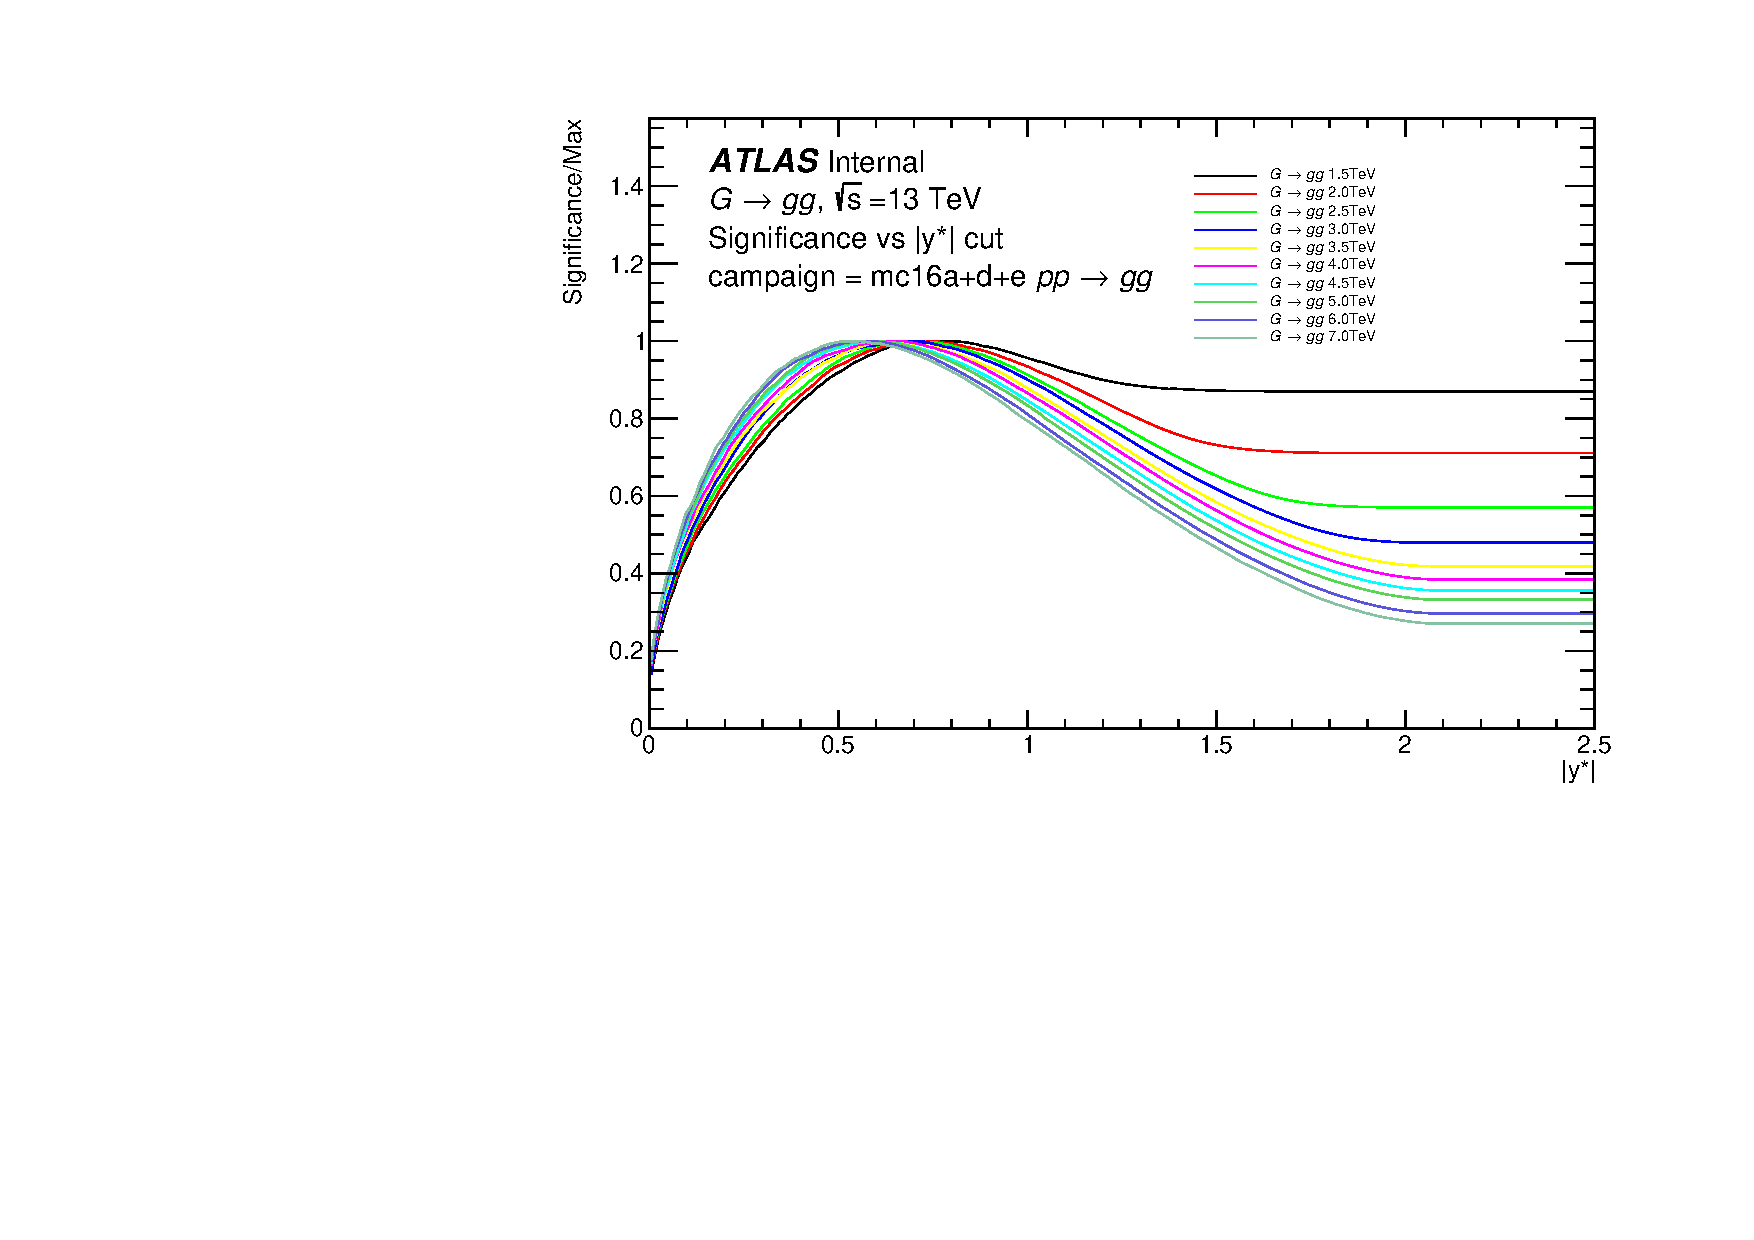
\includegraphics[width=0.45\columnwidth]{fig/yStarOptimization/New_Plots/Significance_Graviton_mc16a+d+e_gg.pdf}}
        \caption{Graviton significance as a function \ystar\ cut in the case of (a) Inclusive, (b) $\geq$1 g-tag, (c) 2 g-tag.}
        \label{fig: graviton significance as a function of y* cut}
\end{figure}


\begin{table}[!htb]
\begin{center}
\begin{tabular}{ccccc}
\toprule
\multicolumn{1}{c}{Graviton Mass (TeV) } & \multicolumn{3}{c}{Optimal Selection} & \multicolumn{1}{c}{Peak Width} \\
& \multicolumn{1}{c|}{Inclusive} & \multicolumn{1}{c|}{$\geq1$ $g$ tag} & \multicolumn{1}{c}{2 $g$ tag} \\
\midrule
1.5 & 0.77 & 0.77 & 0.78 & 0.65\text{--}0.87 \\
2.0 & 0.71 & 0.74 & 0.72 & 0.65\text{--}0.83 \\
2.5 & 0.67 & 0.69 & 0.70 & 0.61\text{--}0.80 \\
3.0 & 0.66 & 0.66 & 0.66 & 0.60\text{--}0.77 \\
3.5 & 0.64 & 0.65 & 0.65 & 0.57\text{--}0.73 \\
4.0 & 0.63 & 0.64 & 0.64 & 0.55\text{--}0.73 \\
4.5 & 0.59 & 0.59 & 0.59 & 0.53\text{--}0.69 \\
5.0 & 0.59 & 0.59 & 0.59 & 0.50\text{--}0.69 \\
6.0 & 0.57 & 0.57 & 0.60 & 0.49\text{--}0.66 \\
7.0 & 0.53 & 0.53 & 0.56 & 0.47\text{--}0.63 \\
\bottomrule
\end{tabular}
\end{center}
\caption{$|y^*|$ selection leading to the maximum significance value calculated using Equation~\ref{eq:signifcanceYstar}.}\label{tab:ystargraviton}
\end{table}



Figure.~\ref{fig: qbh significance as a function of y* cut} shows the significance of QBH signal as a function of \ystar\ cut. The maximum significance is at about 0.9, so the optimal cut for the QBH search is $|\ystar| < 0.9$. Table~\ref{tab:ystarqbh} shows the \ystar\ cut corresponding to the peak significance value for the QBH at each mass point, and the range in \ystar\ cut around the peak that gives a significance $\geq$ 0.99
\begin{figure}[!htb]
        \centering
        \subfloat[Inclusive]{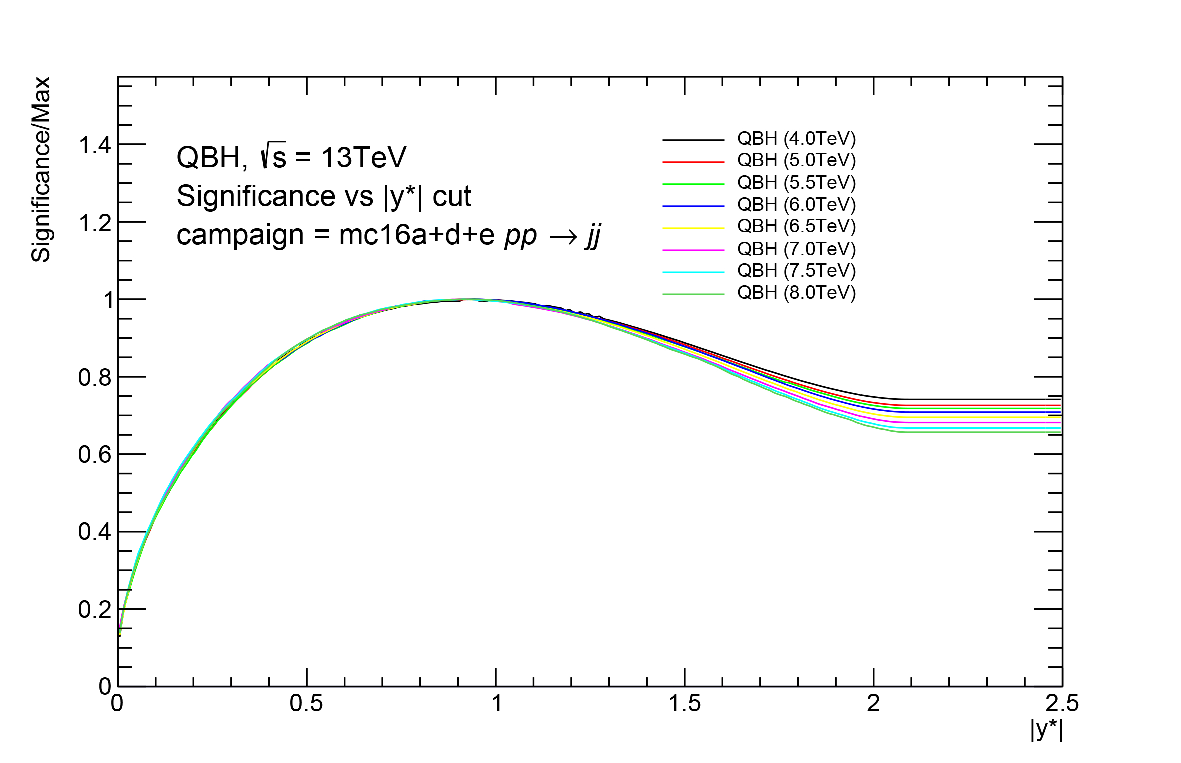
\includegraphics[width=0.45\columnwidth]{fig/yStarOptimization/New_Plots/Significance_QBH_mc16a+d+e_jj.pdf}}
        \subfloat[$\geq$1 g-tag]{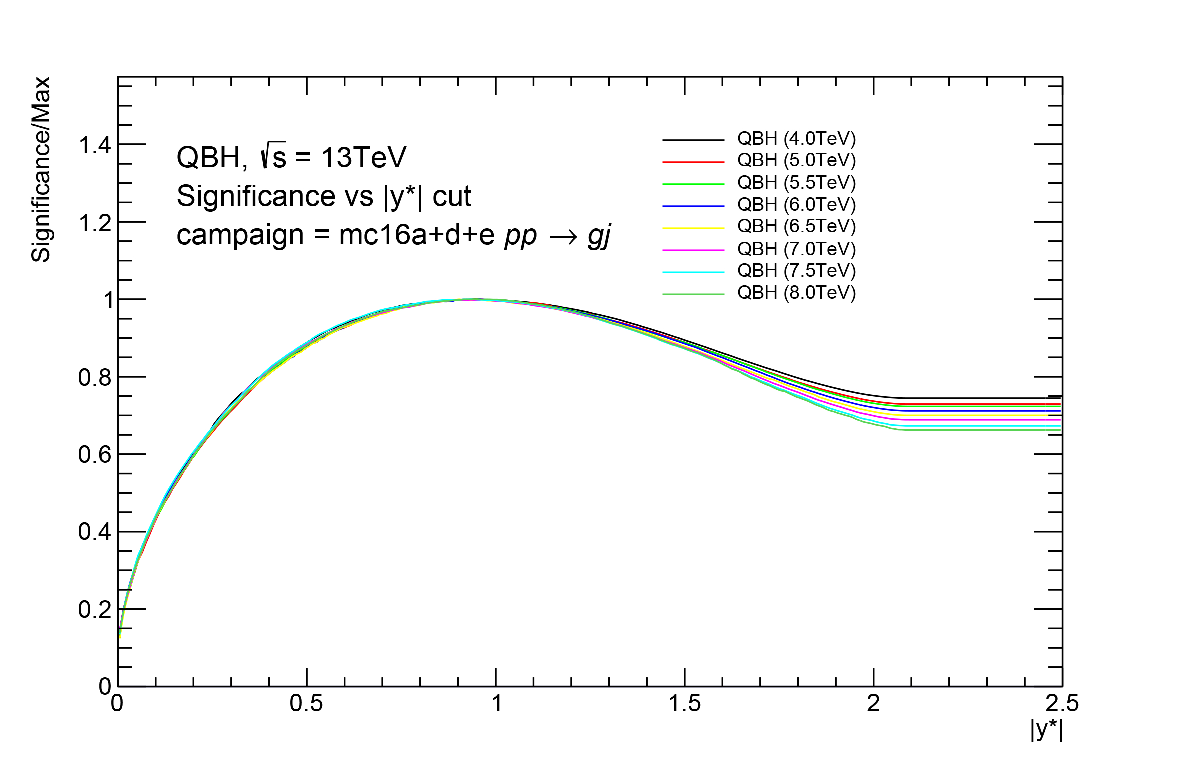
\includegraphics[width=0.45\columnwidth]{fig/yStarOptimization/New_Plots/Significance_QBH_mc16a+d+e_gj.pdf}}\\
        \subfloat[2 g-tag]{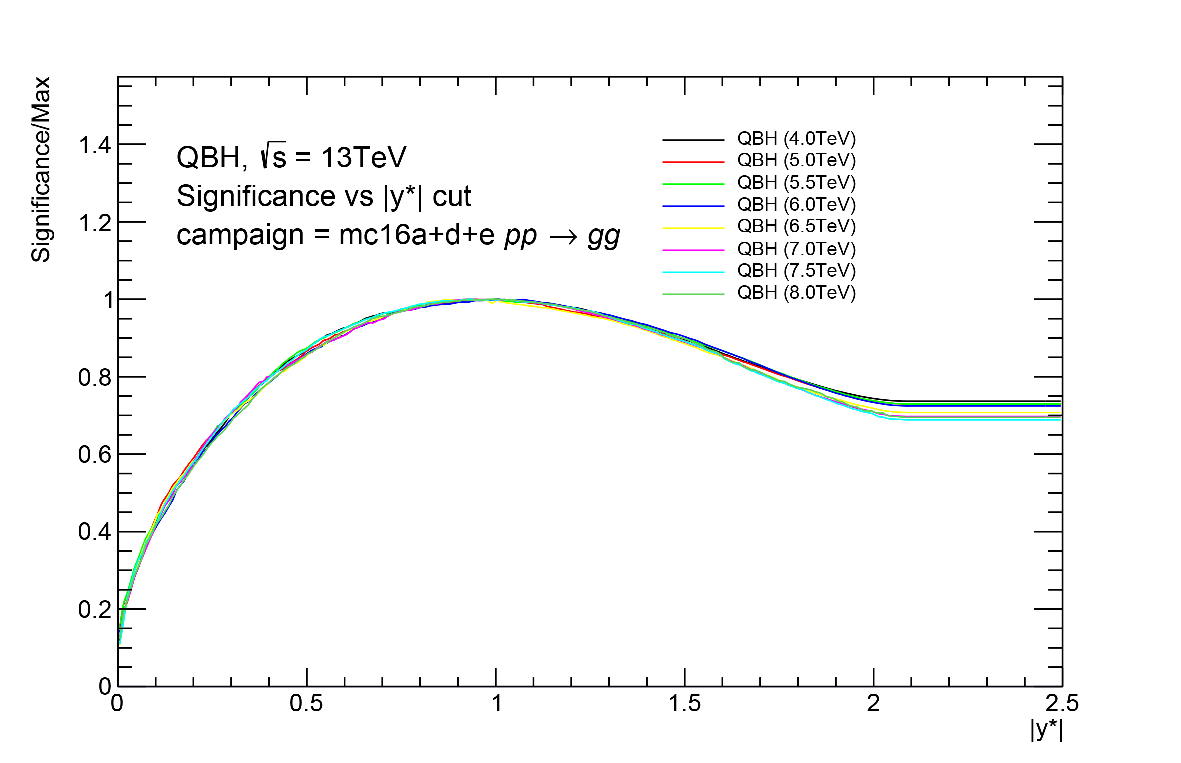
\includegraphics[width=0.45\columnwidth]{fig/yStarOptimization/New_Plots/Significance_QBH_mc16a+d+e_gg.pdf}}
        \caption{QBH significance as a function \ystar\ cut in the case of (a) Inclusive, (b) $\geq$1 g-tag, (c) 2 g-tag.}
        \label{fig: qbh significance as a function of y* cut}
\end{figure}


\begin{table}[!htb]
\begin{center}
\begin{tabular}{ccccc}
\toprule
\multicolumn{1}{c}{QBH Mass (TeV) } & \multicolumn{3}{c}{Optimal Selection} & \multicolumn{1}{c}{Peak Width} \\
& \multicolumn{1}{c|}{Inclusive} & \multicolumn{1}{c|}{$\geq1$ $g$ tag} & \multicolumn{1}{c}{2 $g$ tag} \\
\midrule
4.0 & 0.92 & 0.95 & 1.01 & 0.81\text{--}1.11 \\
5.0 & 0.95 & 0.95 & 0.95 & 0.81\text{--}1.09 \\
5.5 & 0.94 & 0.96 & 0.94 & 0.81\text{--}1.09 \\
6.0 & 0.92 & 0.96 & 1.01 & 0.81\text{--}1.09 \\
6.5 & 0.91 & 0.91 & 0.93 & 0.81\text{--}1.06 \\
7.0 & 0.93 & 0.97 & 0.94 & 0.82\text{--}1.07 \\
7.5 & 0.92 & 0.94 & 0.93 & 0.79\text{--}1.08 \\
8.0 & 0.92 & 0.96 & 0.99 & 0.82\text{--}1.09 \\
\bottomrule
\end{tabular}
\end{center}
\caption{$|y^*|$ selection leading to the maximum significance value calculated using Equation~\ref{eq:signifcanceYstar}.}\label{tab:ystarqbh}
\end{table}

However, further study have provided that using multiple signal regions was an over optimisation, so in the analysis, $|y^*|$ < 0.8 is used.

\FloatBarrier
%
%\subsubsection{Dijet Mass Turn-on}
%\label{section:dijetmassturn-on} % uncomment if label used.
%
%The \mjj\ turn-on is investigated by comparing events collected with the highest \pt\ 
%trigger threshold with one with a lower \pt\ threshold using data. The efficiency of the HLT\_j420 trigger is calculated by comparing to the following triggers in each data taking period: 2015 HLT\_j360, 2016 HLT\_j380, 2017 and 2018 HLT\_mu50.  The muon trigger 2017 and 2018 are included as HLT\_j420 is the only unprescaled jet trigger available. The full Run 2 dataset is included for comparison as the HLT\_mu50 is available for all running periods. Events where the efficiency of trigger less than 99.5\% will be removed by a mass cut.
%
%
%The efficiencies as a function of \mjj\ are shown in Figure.~\ref{fig: mass turn-on yStar 0.6} for $|\ystar|<0.6$ and Figure.~\ref{fig: mass turn-on yStar 0.8} for $|\ystar|<0.8$ in two gluon-tag categories for both triggers.  The results are summarised in Table.~\ref{table:massTurnOns} for the different data-taking periods. The \mjj~mass cut is chosen to be slightly above the value of the plateau ($\geq$99.5\%), so a cut of 1100 GeV
%for $|\ystar|<0.6$ is applied. For $|\ystar|<0.8$, a cut of 1200 GeV is applied to samples with either one or two gluon tags.
%
%\begin{figure}[htbp]
%        \centering
%        \subfloat[$\geq$1 g-tag]{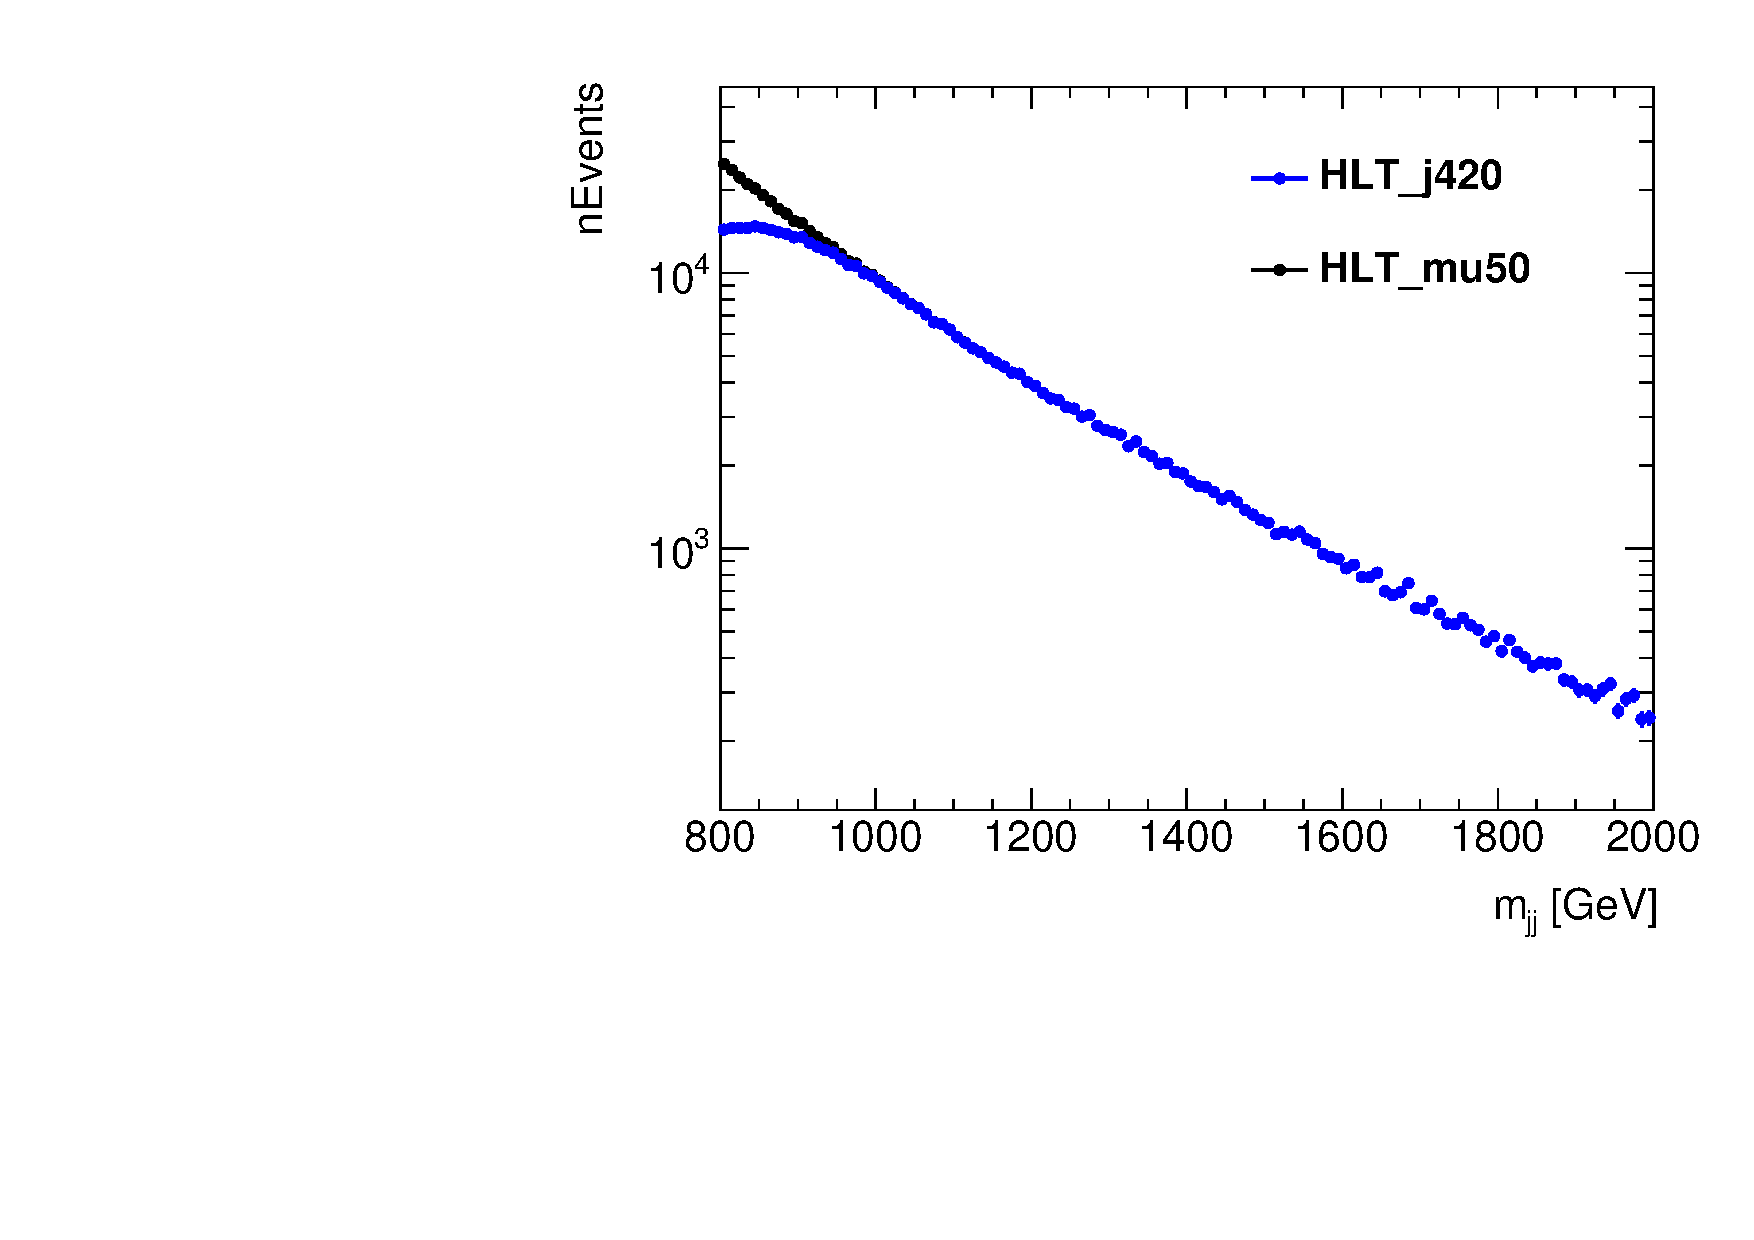
\includegraphics[width=0.5\columnwidth]{fig/massturnon/yStar0p6/mjj_turnon_1gluonTag_yStar0p6}}
%        \subfloat[2 g-tag]{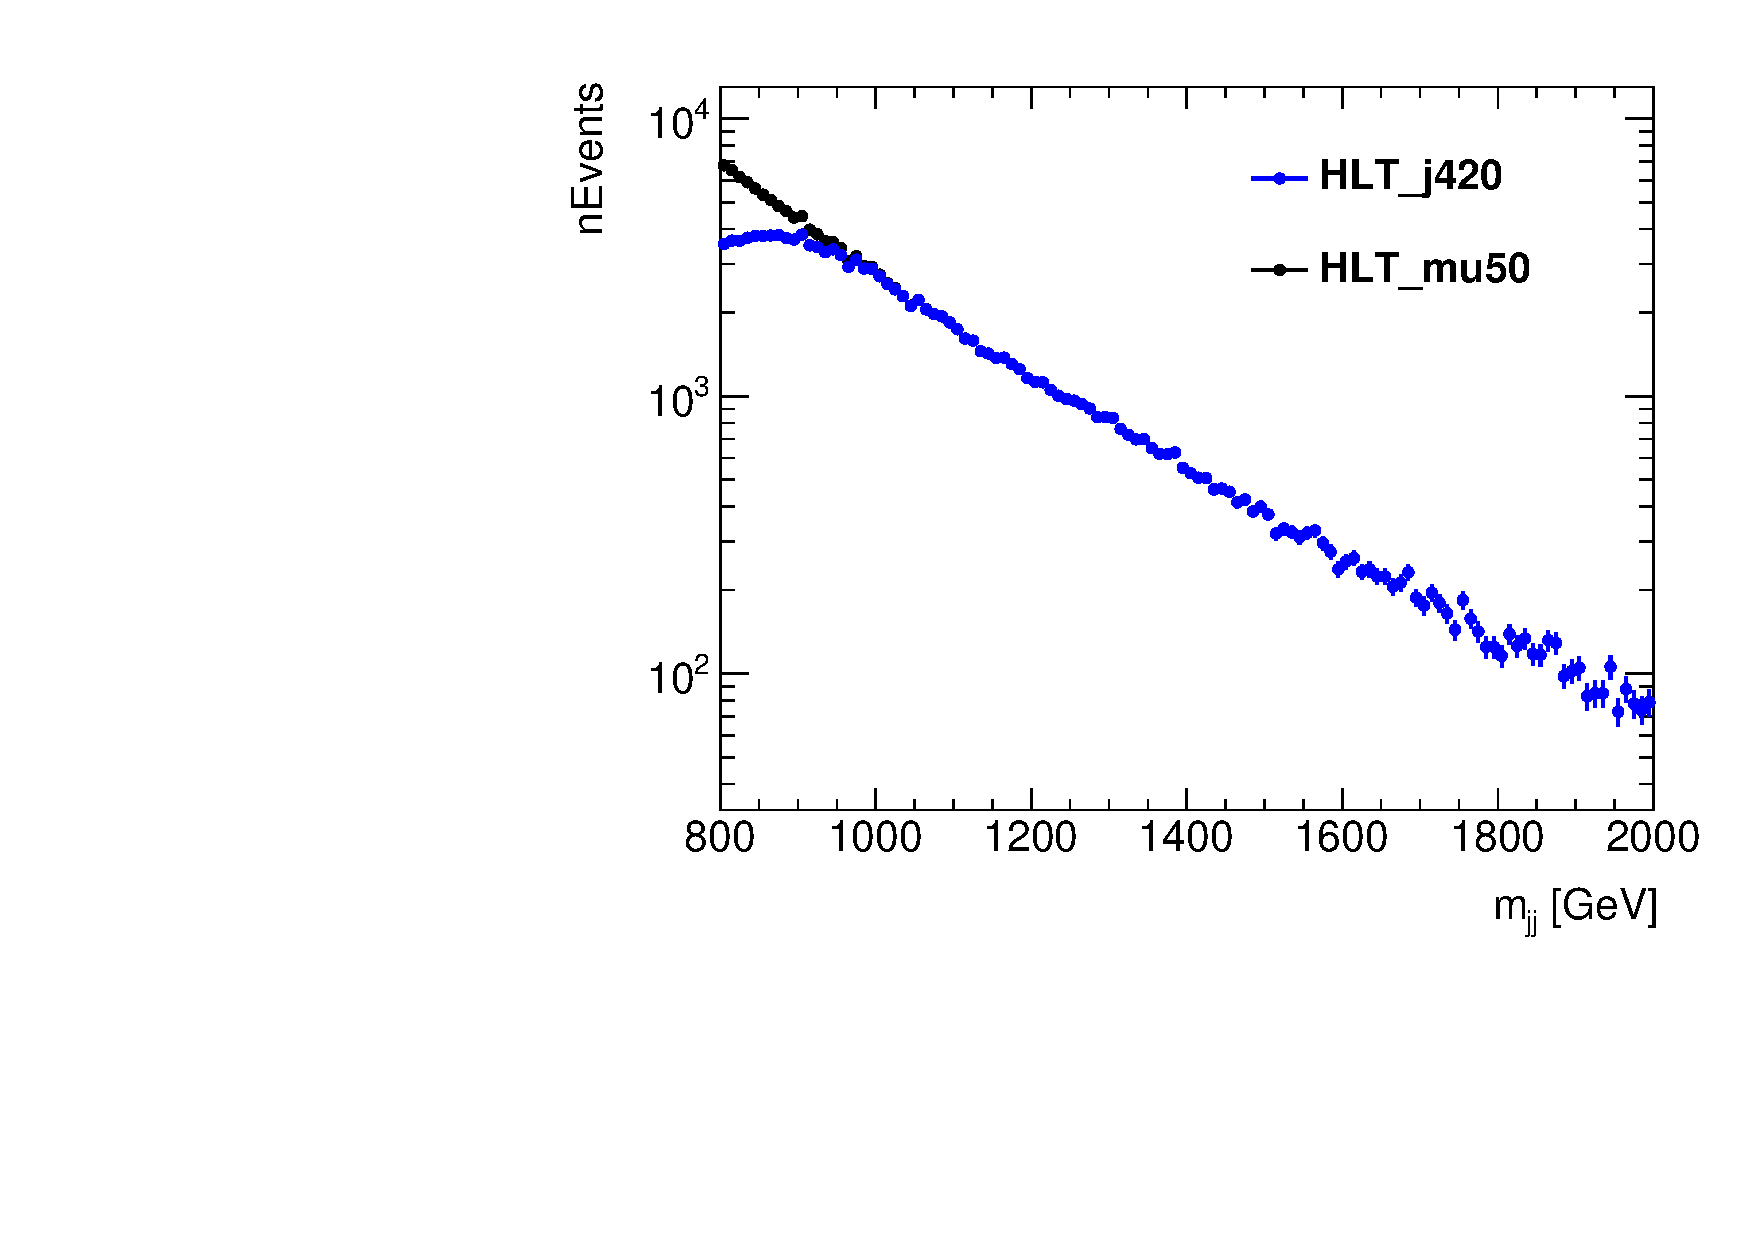
\includegraphics[width=0.5\columnwidth]{fig/massturnon/yStar0p6/mjj_turnon_2gluonTag_yStar0p6}}
%        \\
%        \subfloat[$\geq$1 g-tag]{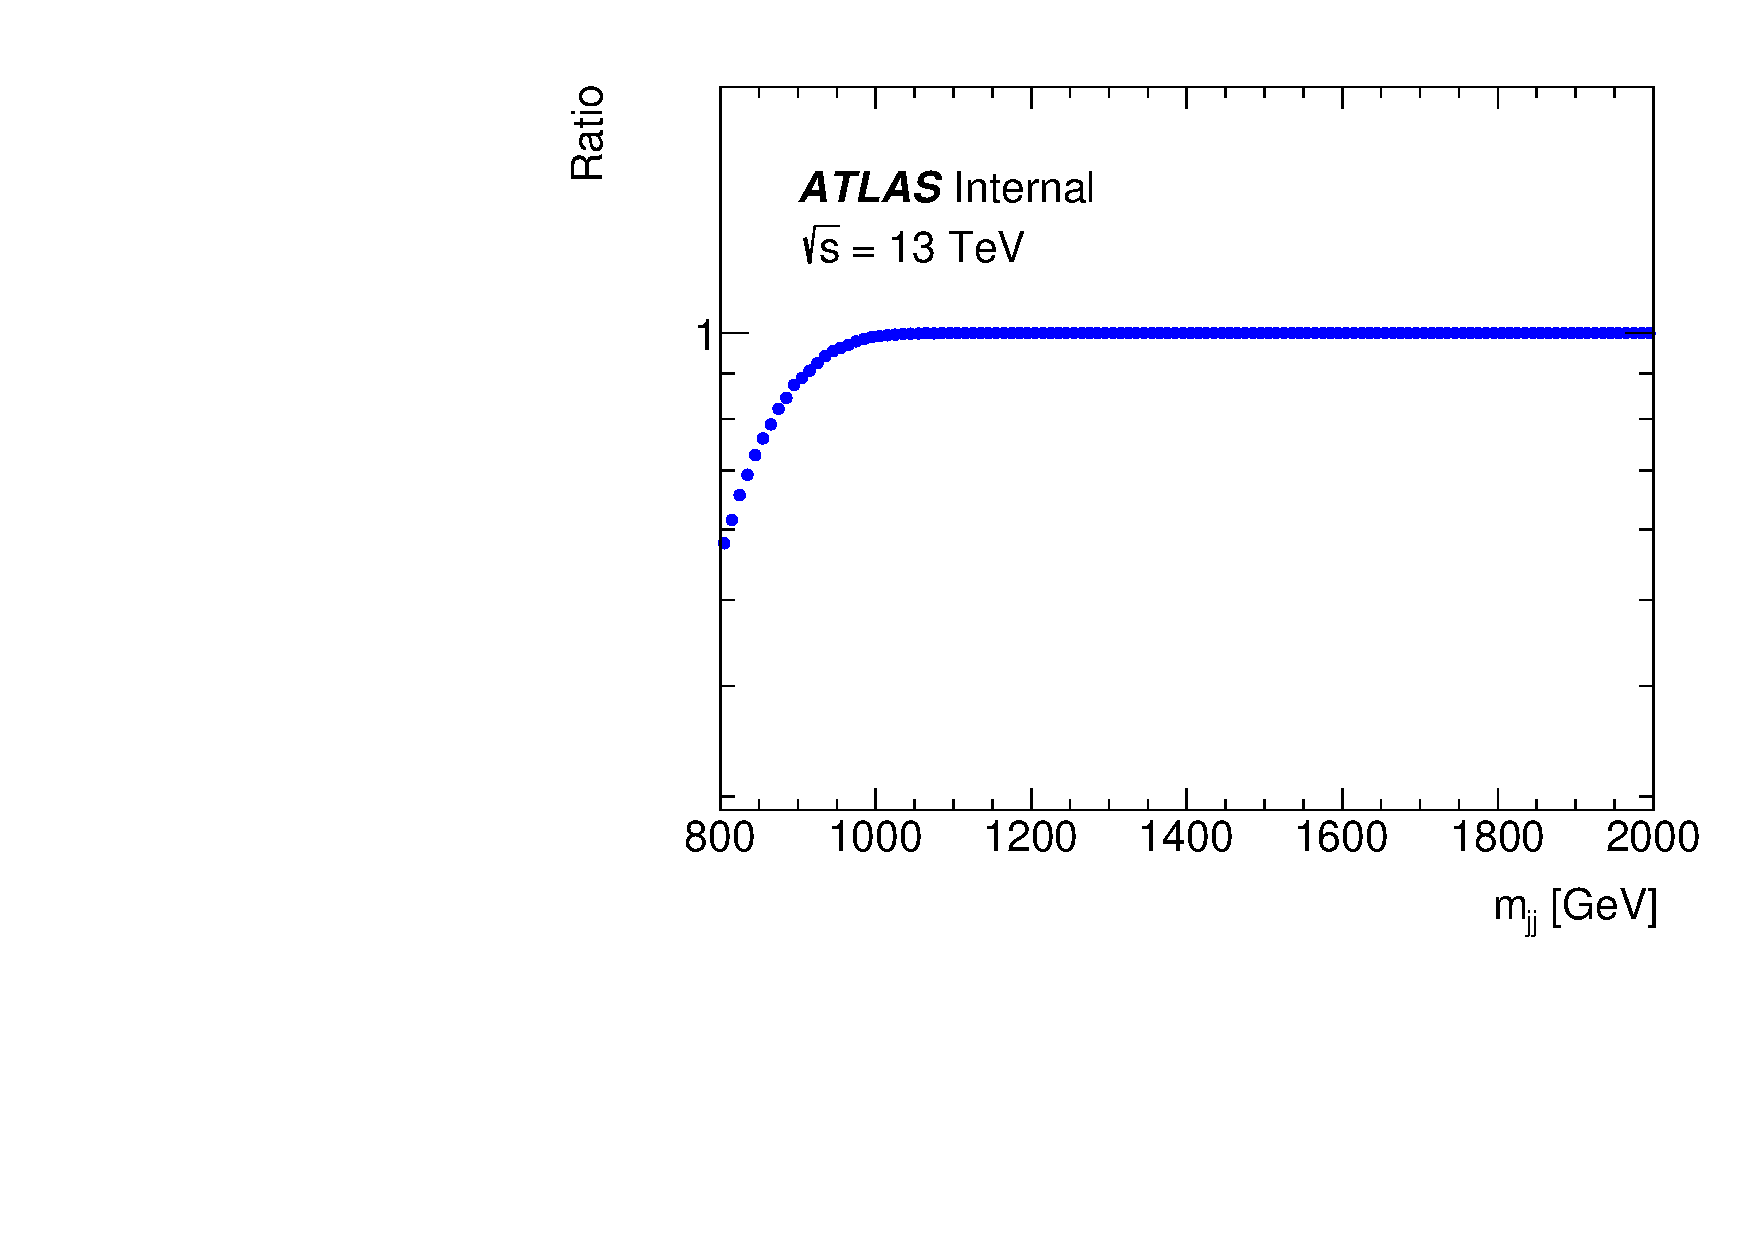
\includegraphics[width=0.5\columnwidth]{fig/massturnon/yStar0p6/Ratio_mjj_turnon_1gluonTag_yStar0p6}}
%        \subfloat[2 g-tag]{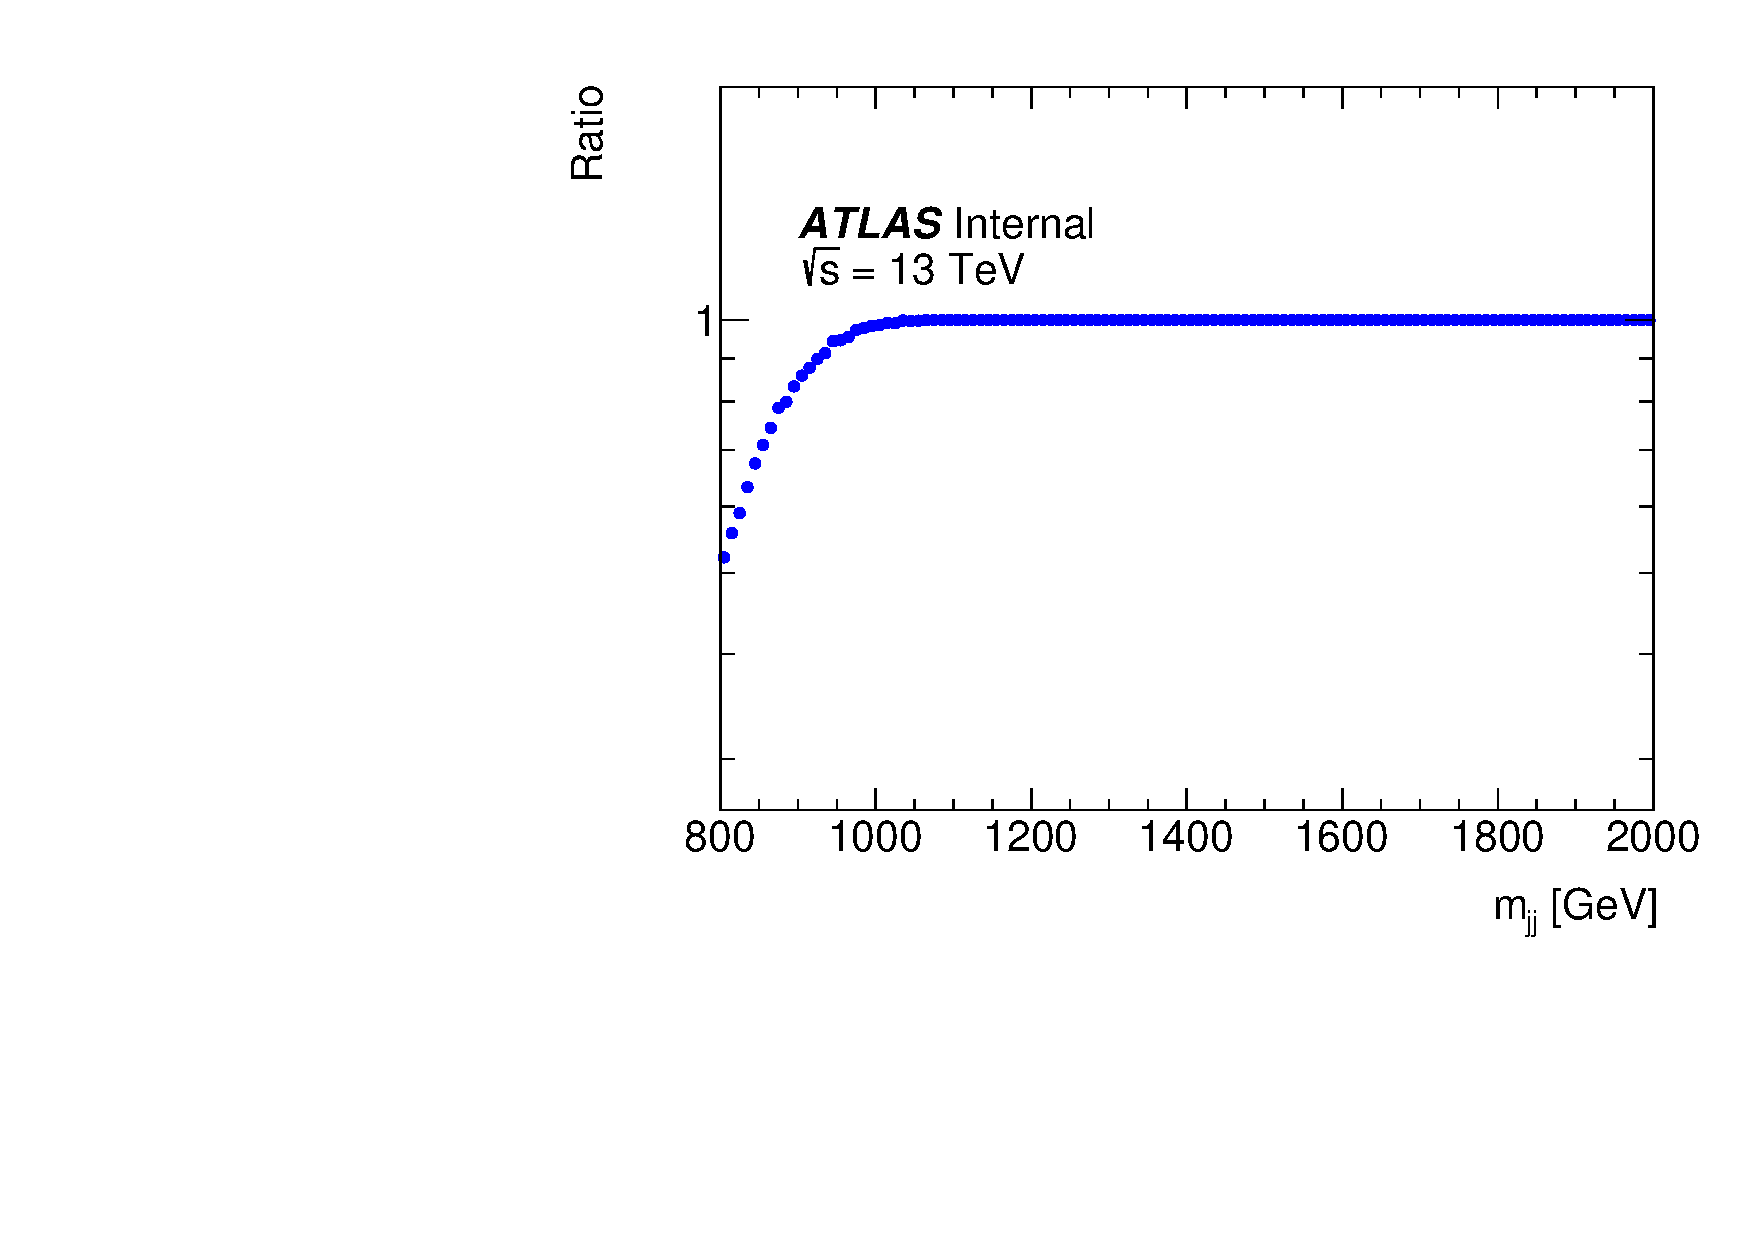
\includegraphics[width=0.5\columnwidth]{fig/massturnon/yStar0p6/Ratio_mjj_turnon_2gluonTag_yStar0p6}}
%        
%        \caption{Efficiencies as a function of \mjj\ for $|\ystar|<0.6$ using HLT\_j420 compared with HLT\_mu50 in the case of comparison of mass spectra with 
%        (a) $\geq$1 g-tag, (b) 2 g-tag and the ratio between the two (c) $\geq$1 g-tag and (d) 2 g-tag.}
%        \label{fig: mass turn-on yStar 0.6}
%\end{figure}
%
%\begin{figure}[htbp]
%        \centering
%        \subfloat[$\geq$1 g-tag]{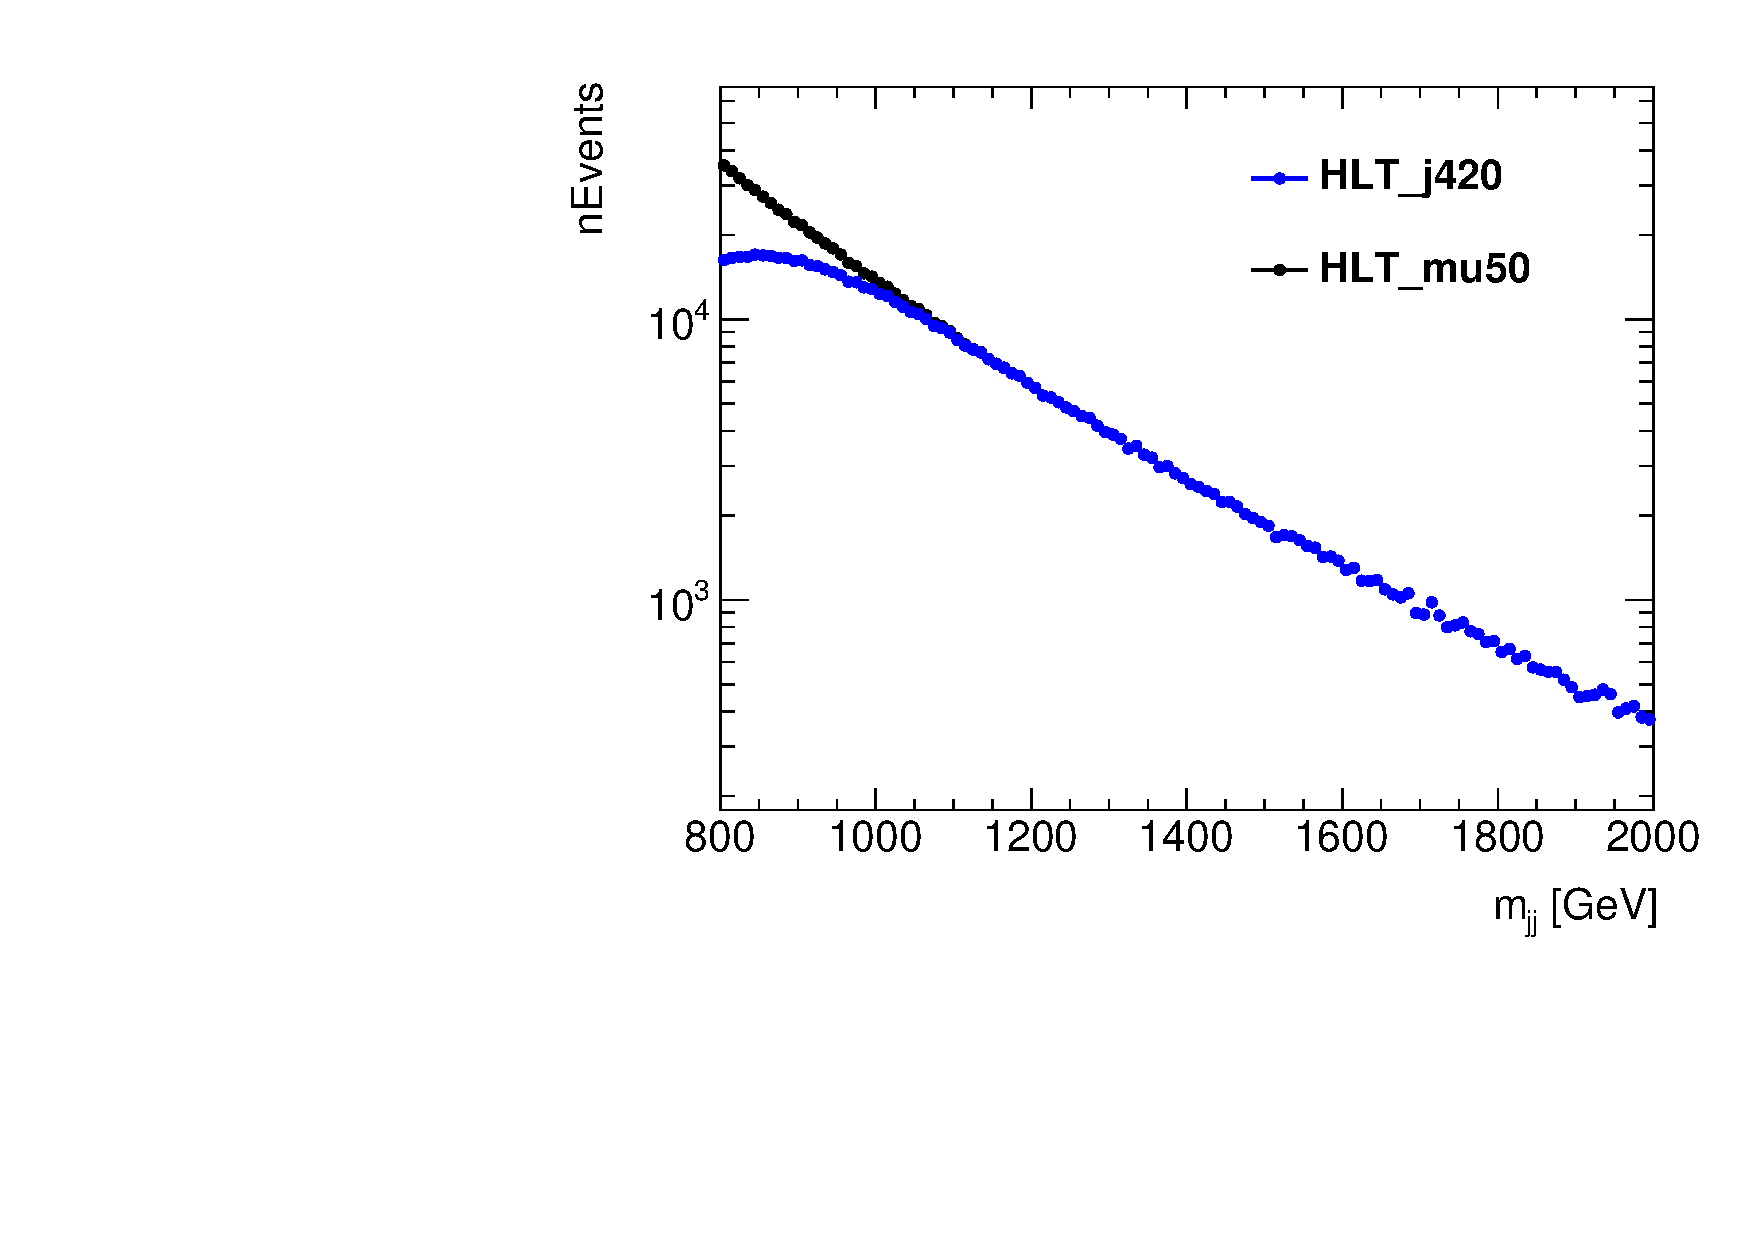
\includegraphics[width=0.5\columnwidth]{fig/massturnon/yStar0p8/mjj_turnon_1gluonTag_yStar0p8}}
%        \subfloat[2 g-tag]{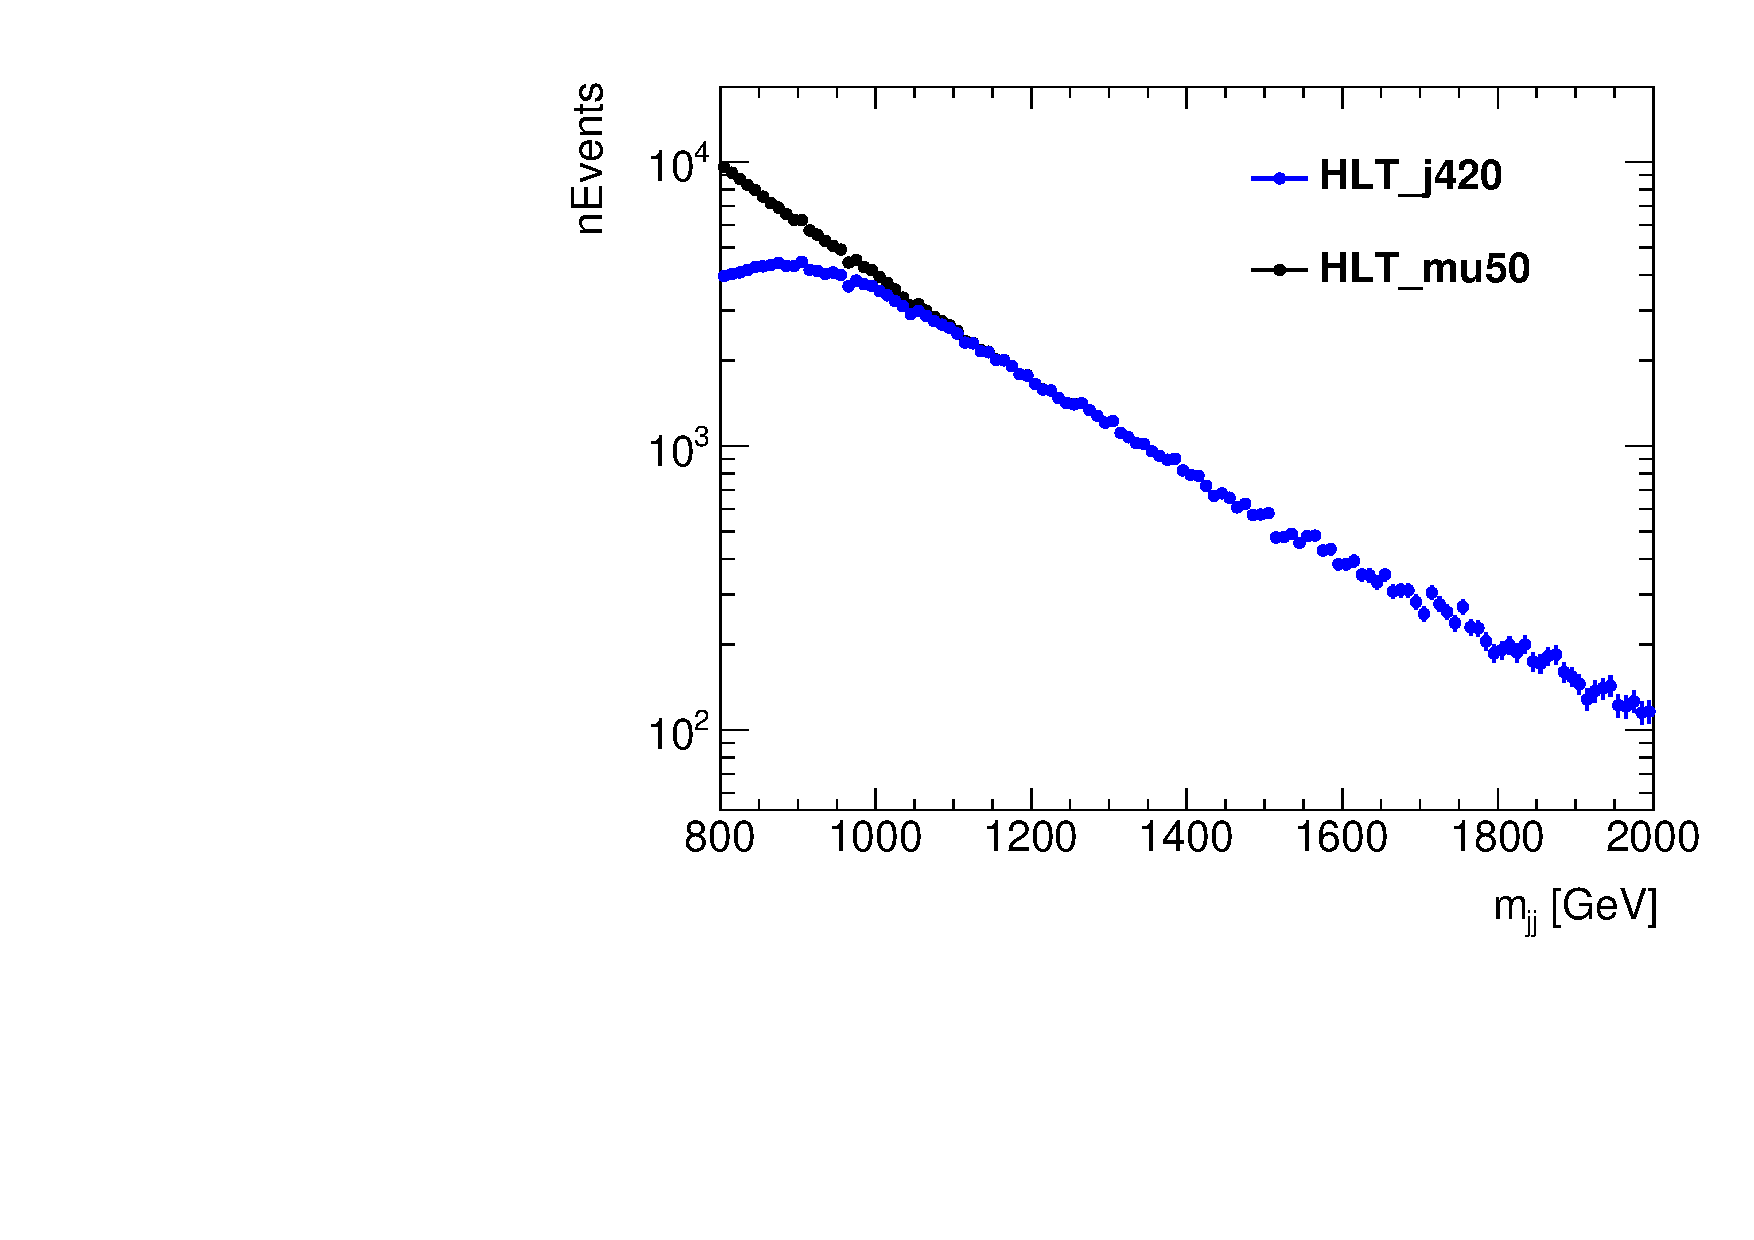
\includegraphics[width=0.5\columnwidth]{fig/massturnon/yStar0p8/mjj_turnon_2gluonTag_yStar0p8}}
%        \\
%        \subfloat[$\geq$1 g-tag]{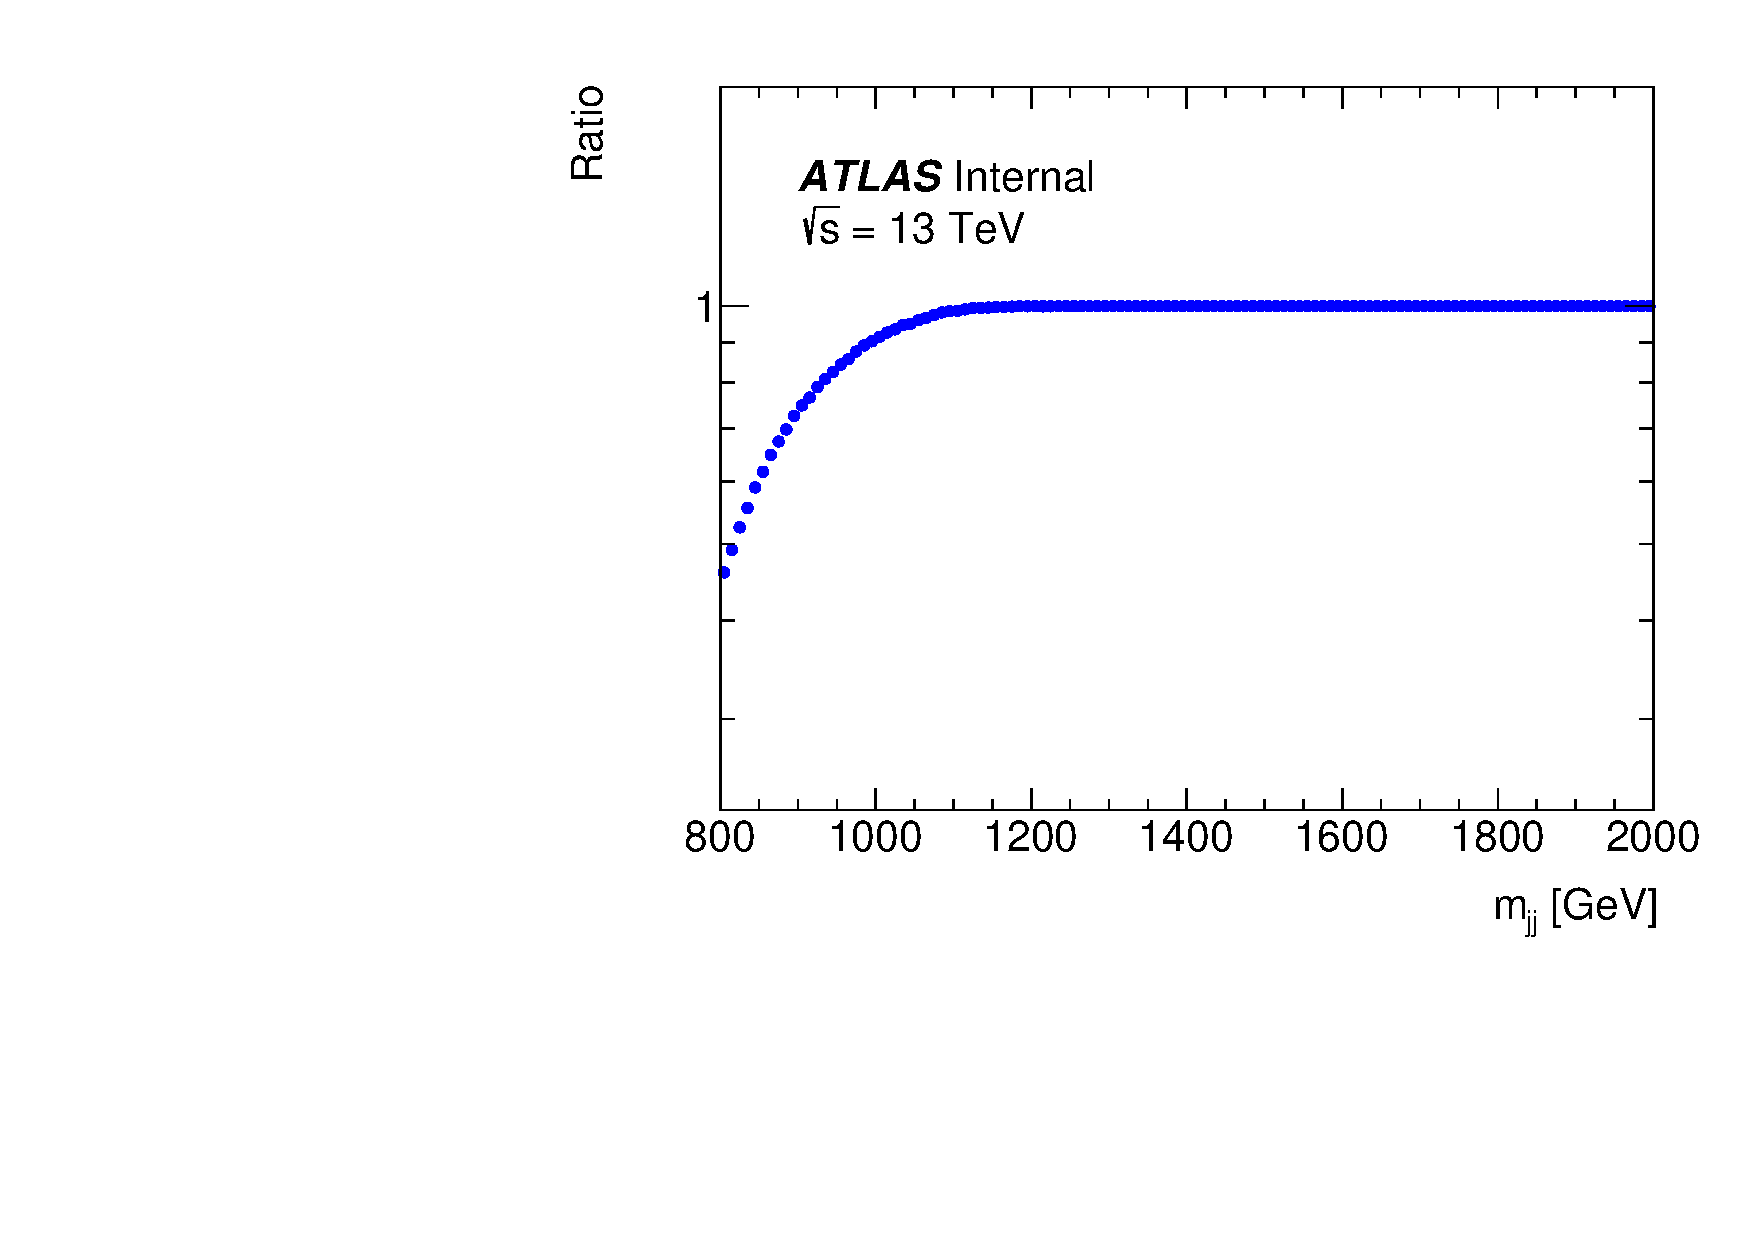
\includegraphics[width=0.5\columnwidth]{fig/massturnon/yStar0p8/Ratio_mjj_turnon_1gluonTag_yStar0p8}}
%        \subfloat[2 g-tag]{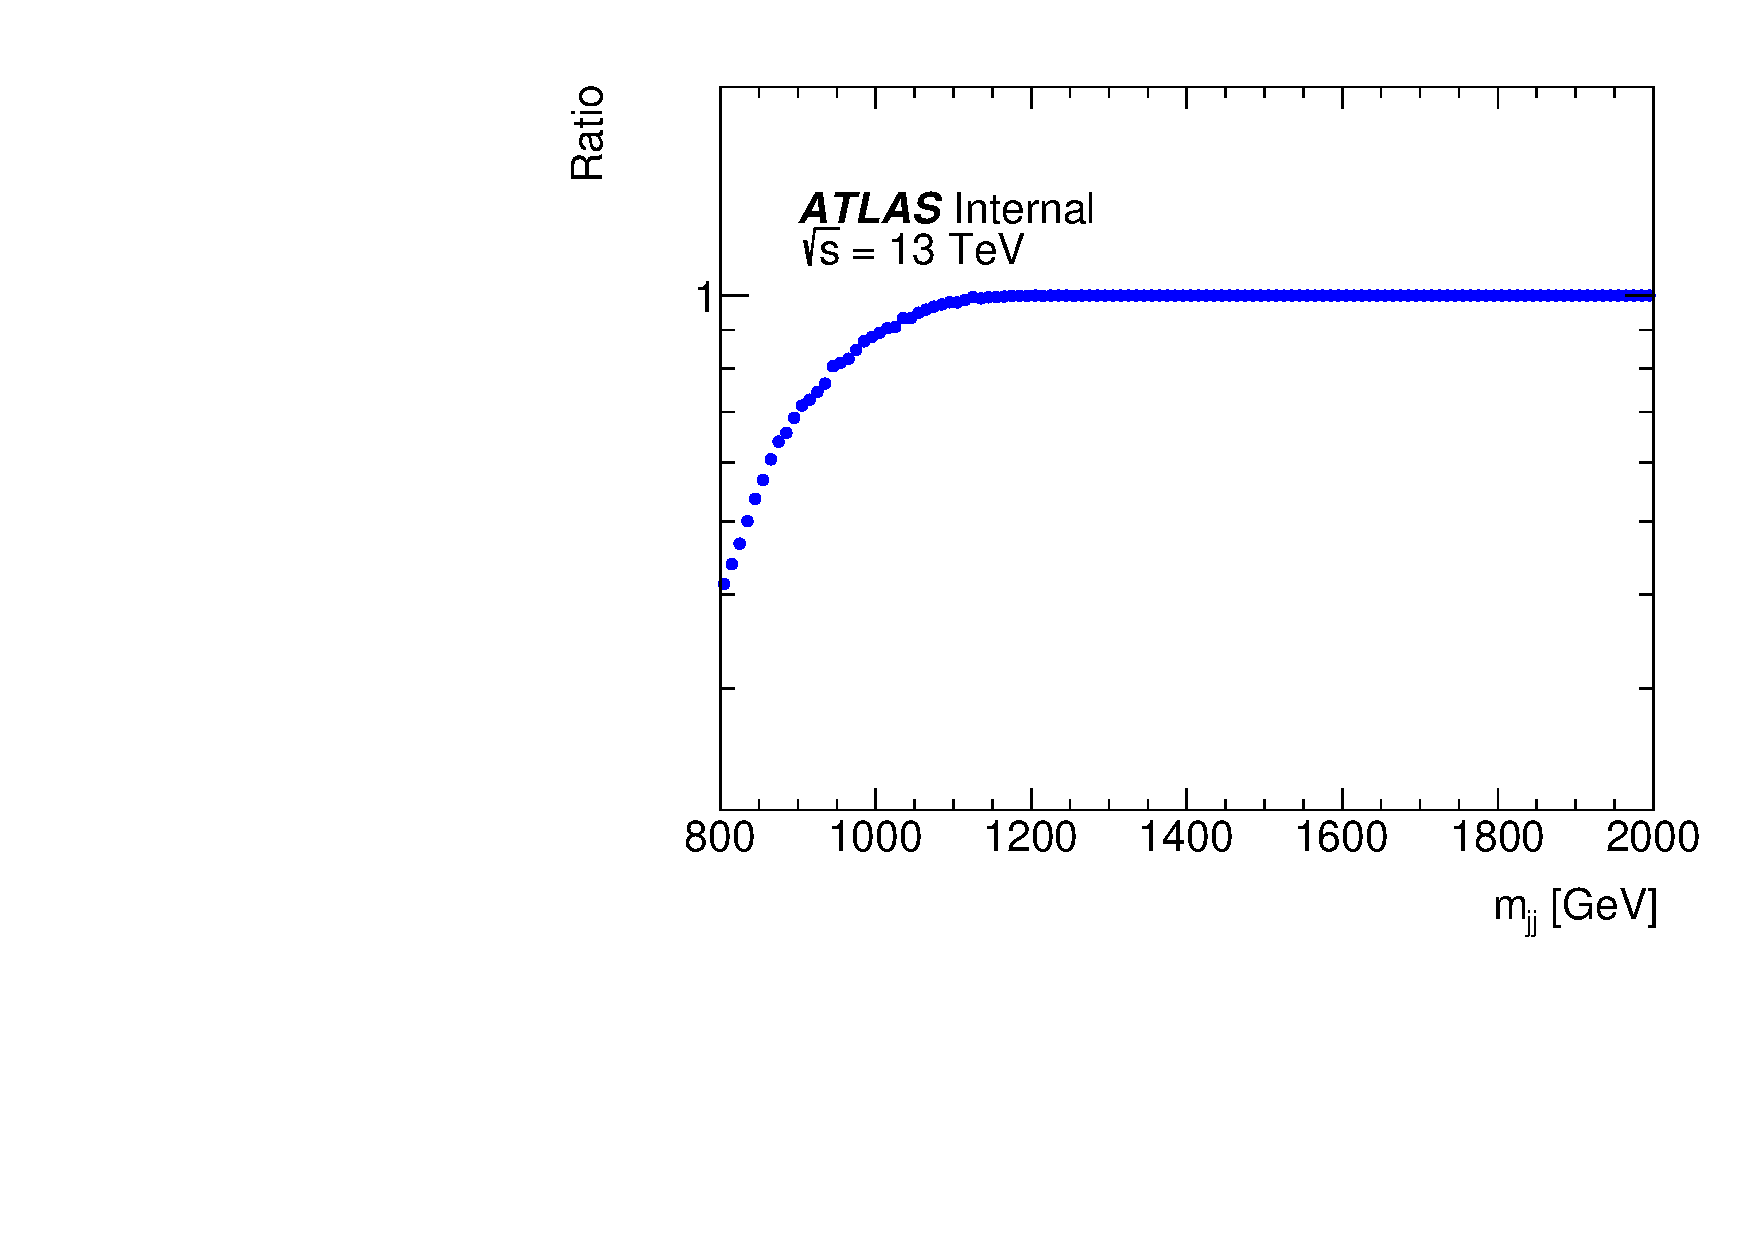
\includegraphics[width=0.5\columnwidth]{fig/massturnon/yStar0p8/Ratio_mjj_turnon_2gluonTag_yStar0p8}}
%        \caption{Efficiencies as a function of \mjj\ for $|\ystar|<0.8$ using HLT\_j420 compared with HLT\_mu50 in the case of comparison of mass spectra with 
%        (a) $\geq$1 g-tag, (b) 2 g-tag and the ratio between the two (c) $\geq$1 g-tag and (d) 2 g-tag.}
%        \label{fig: mass turn-on yStar 0.8}
%\end{figure}
%
%\begin{table}[h]
%	\centering 
%	\resizebox{0.95\textwidth}{!}{
%	\begin{tabular}{SSSSS}
%		\toprule
%		\multicolumn{1}{c}{Data Taking Period}  &  \multicolumn{2}{c}{Mass turn on $|\ystar|<0.6$ } &  \multicolumn{2}{c}{Mass turn on $|\ystar|<0.8$ } \\
%		& \multicolumn{1}{c}{$\geq$1 g-tag ( GeV )} &  \multicolumn{1}{c}{2 g-tag ( GeV )} 
%		& \multicolumn{1}{c}{$\geq$1 g-tag ( GeV )} &  \multicolumn{1}{c}{2 g-tag ( GeV )}  \\
%		\midrule 
%		2015  & 1040 & 1030 & 1160 & 1160 \\
%		2016  & 1030 & 1030 & 1160 & 1170 \\
%		2017  & 990 & 1000  & 1110 & 1120 \\
%		2018  & 1000 & 1010  & 1110 & 1120 \\
%		\multicolumn{1}{c}{Run~2} & 1020 & 1030 & 1120 & 1120 \\
%		\bottomrule
%	\end{tabular}}
%	\caption{ The \mjj value of the start of the plateau ($\geq$99.5\%) for each period of data taking. 
%		\label{table:massTurnOns}
%	}
%\end{table}
%
%\FloatBarrier
\subsubsection{Optimised selection}
\label{sec:analysiscuts}

In addition to the baseline selection described in Section~\ref{sec:base_selection}, optimized cuts are  applied to different tagging regions to improve the search potential with good tracking efficiency. 

The following additional cuts are applied for the the inclusive samples.
\begin{itemize}
	\item $|\ystar| < 0.8$
	\item \mjj > 1200 GeV
\end{itemize}

The following additional cuts are for quark-gluon tagging.
\begin{itemize}
	\item $|\eta| < 2.1$ (both jets) for track acceptance
	\item $\ge 1$ gluon tagged (75\% working point)
	\item 2 gluons tagged (75\% working point)
\end{itemize}
where the 75\% gluon selection criteria is $n_\mathrm{track} > -13.399 +5.049\ln(\pt)$, with \pt\ in GeV.


\FloatBarrier

%The acceptance times efficiency as a function of signal masses in inclusive, signal-gluon and double-gluon
%tagged regions for different benchmark signal models are shown in Figure~\ref{fig:AccxEff}.
%
%\begin{figure}[htb]
% \centering
% 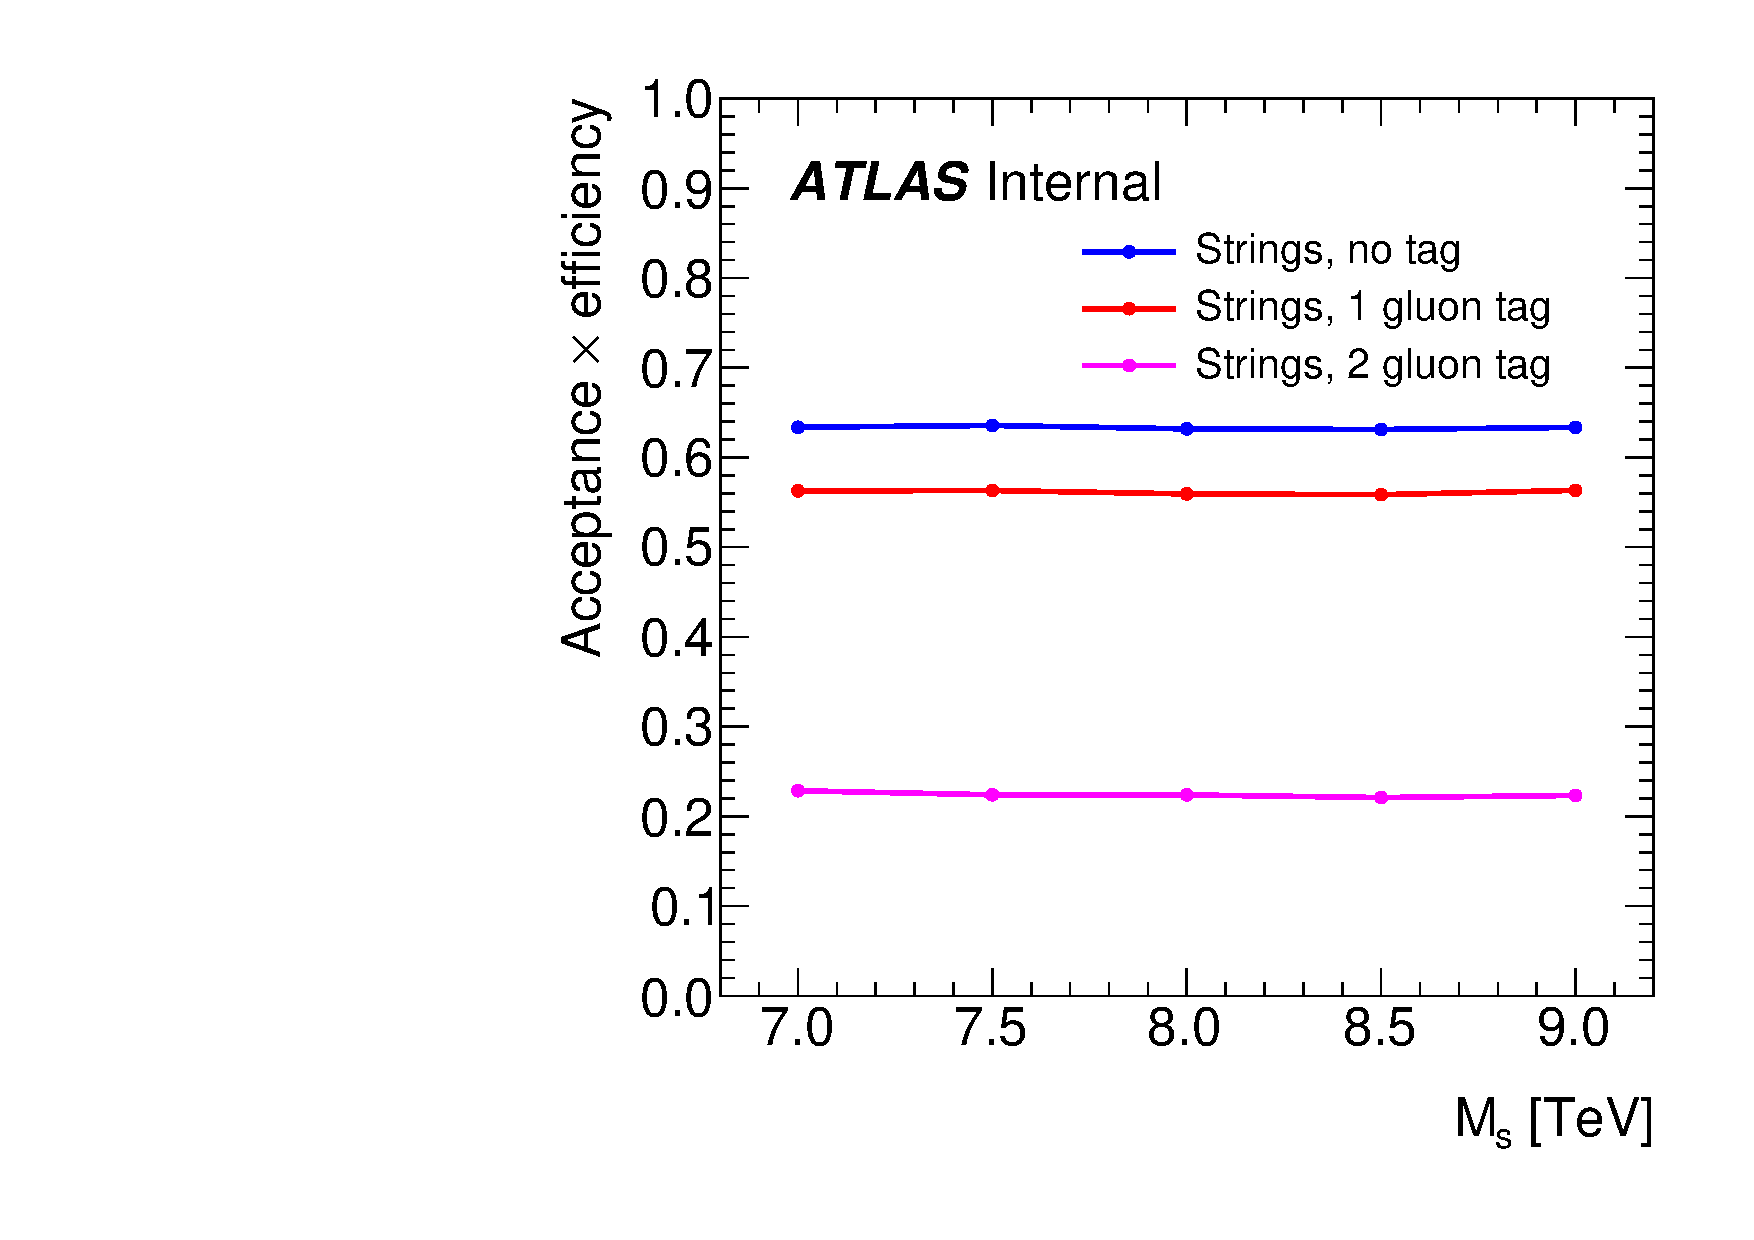
\includegraphics[width=0.5\textwidth]{fig/benchmark_signals/AccxEff_strings.pdf}
% \caption{Acceptance times efficiency for the String signal.}
% \label{fig:AccxEff}
%\end{figure}
%\FloatBarrier
\subsubsection{Selected kinematic plots}
%\label{sec:kinematic_distributions} % uncomment if label used.

In this section a selection of kinematic and monitoring plots processed with samples passed the one- and two-gluon selection criteria are shown in Figure~\ref{fig:GGmonitoring1} to\ref{fig:GGmonitoring4}. 
\begin{figure}[htb]
 \centering
\subfloat[]{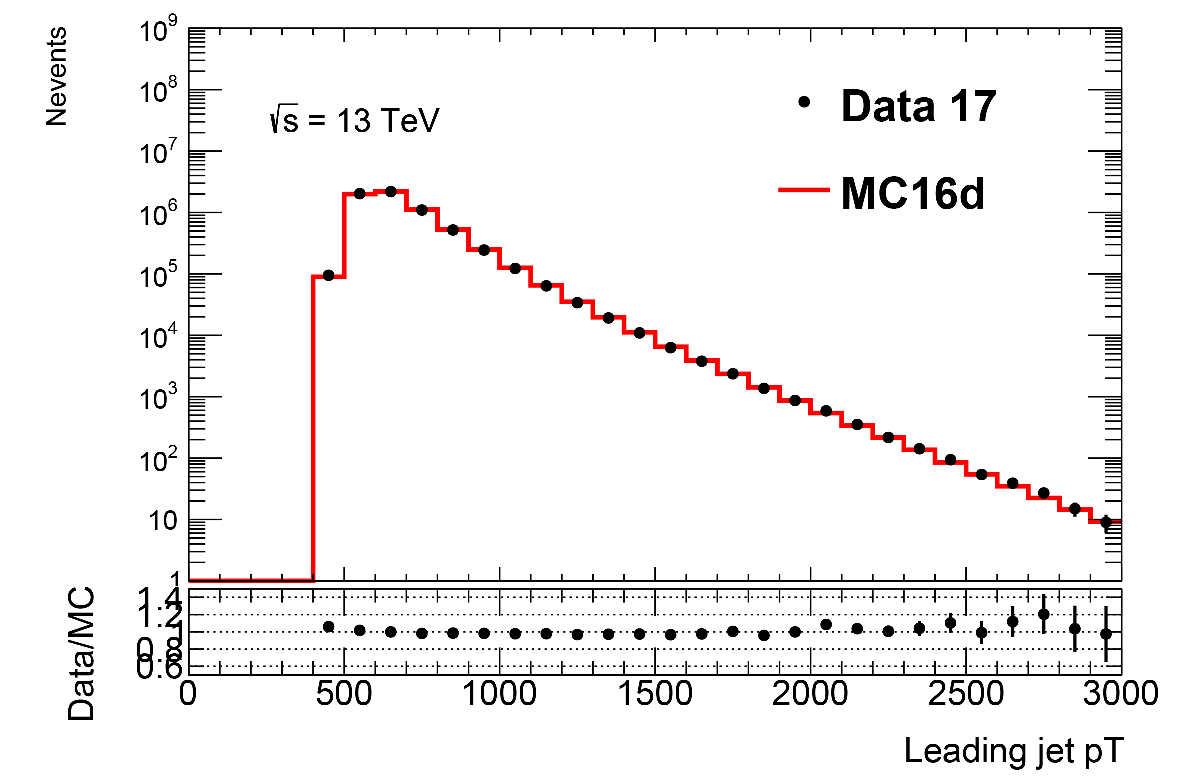
\includegraphics[width=0.45\textwidth]{fig/monitoring/1gtag/MC16d/LeadingJetPt.pdf}}
\subfloat[] {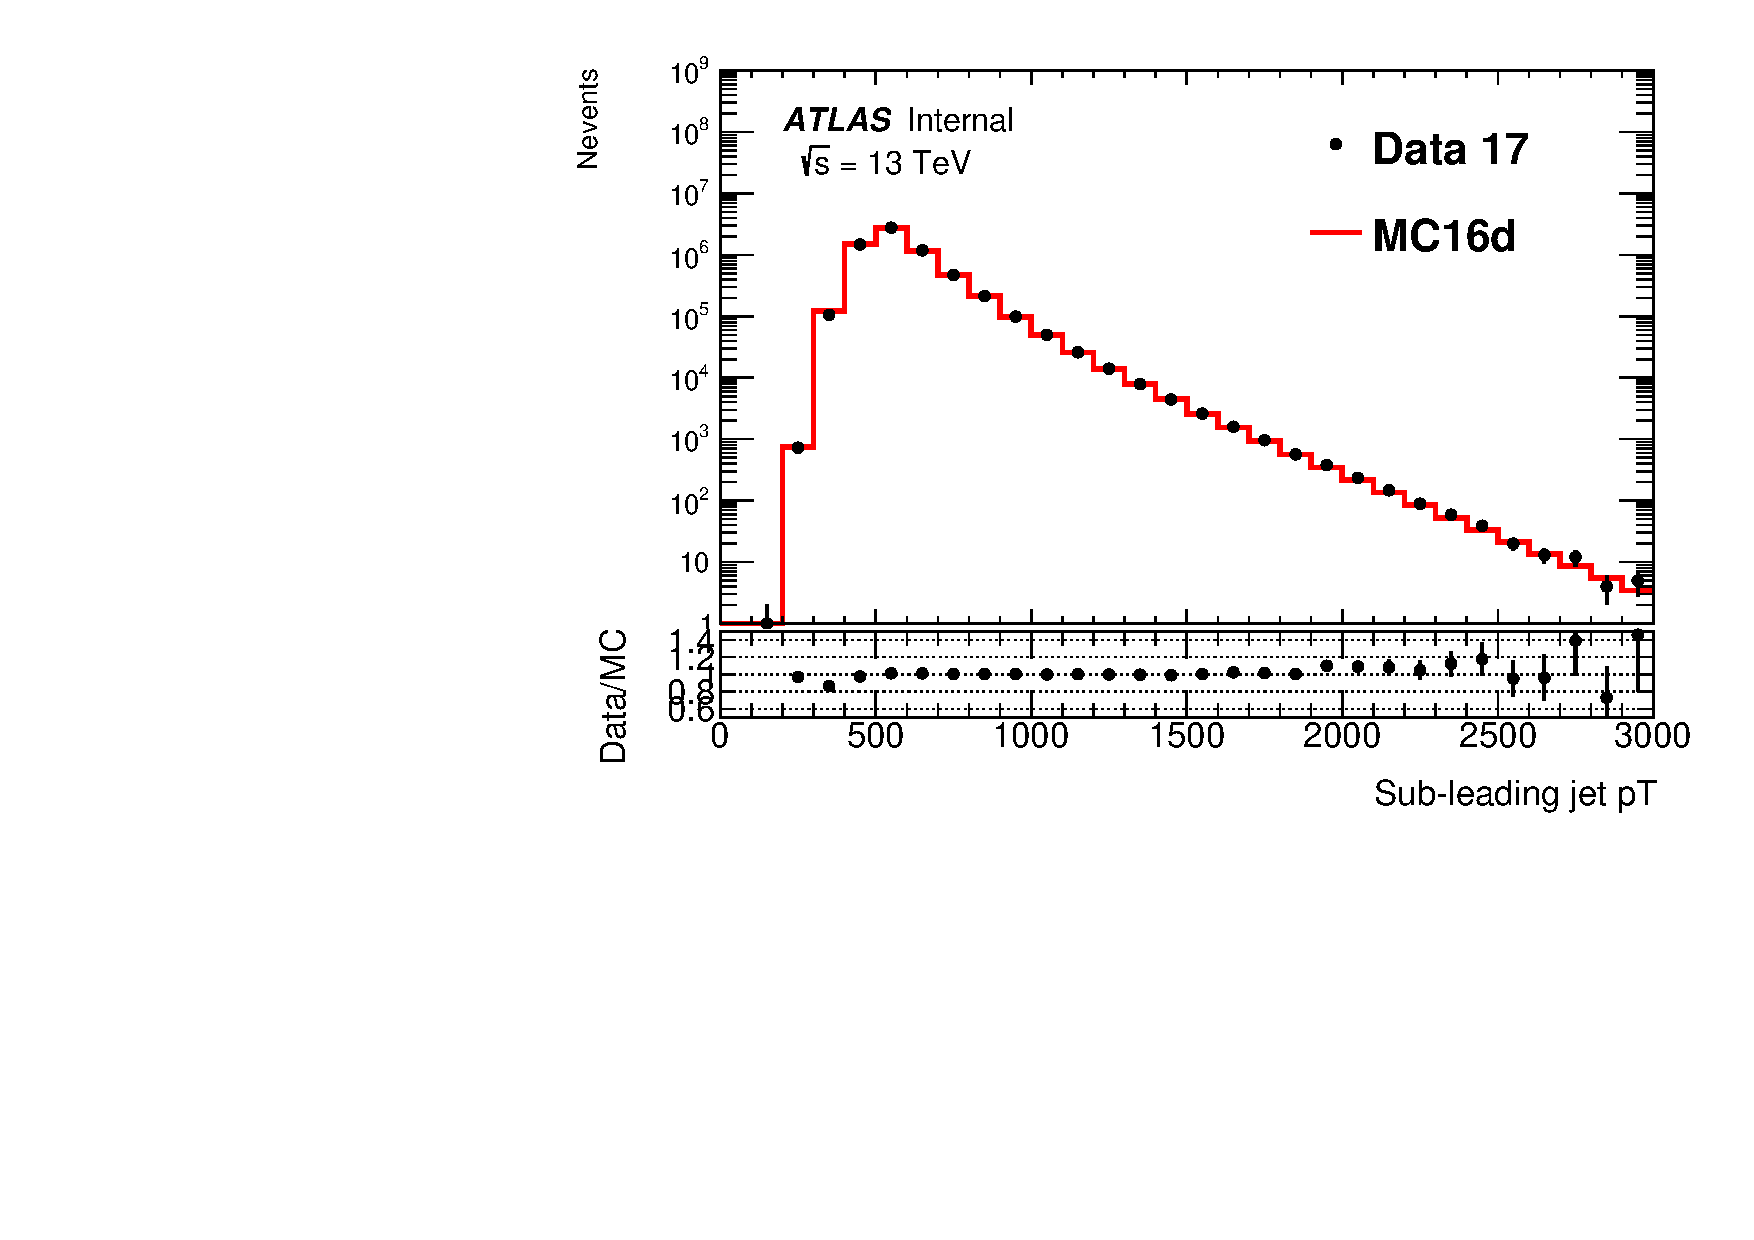
\includegraphics[width=0.45\textwidth]{fig/monitoring/1gtag/MC16d/SubLeadingJetPt.pdf}}\\
\subfloat[] {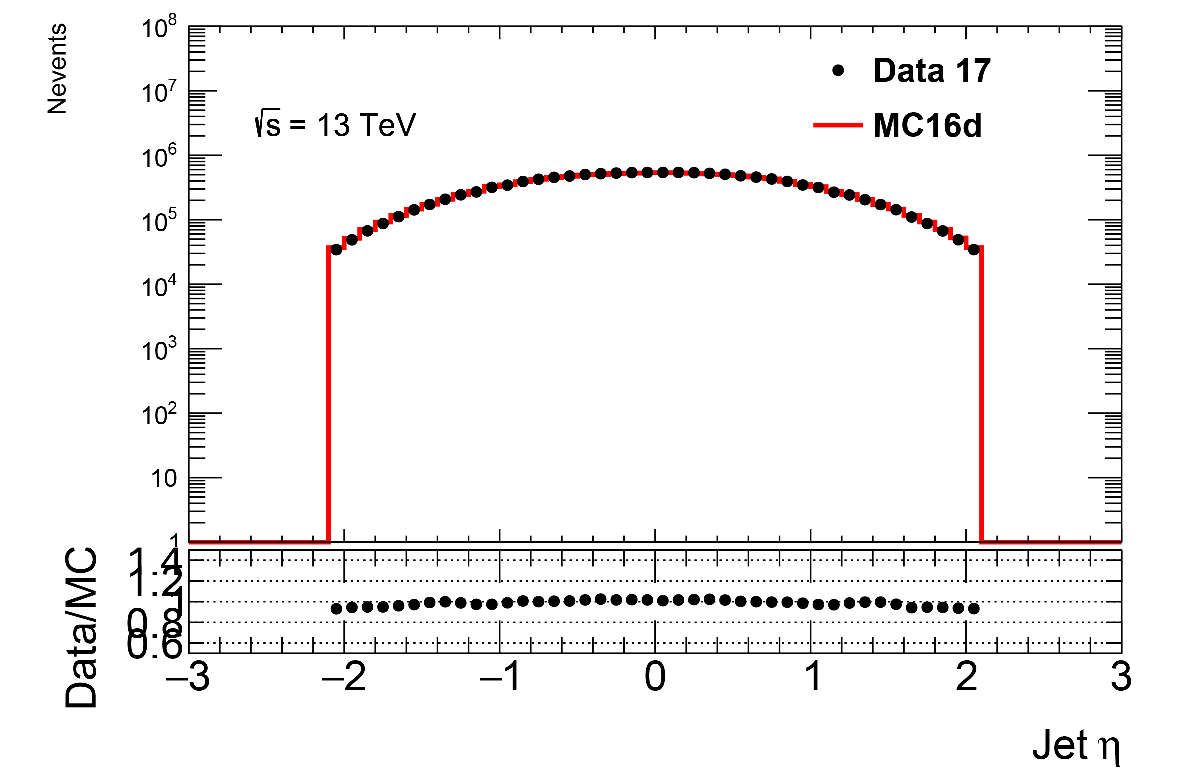
\includegraphics[width=0.45\textwidth]{fig/monitoring/1gtag/MC16d/JetEta.pdf}}
\subfloat[] {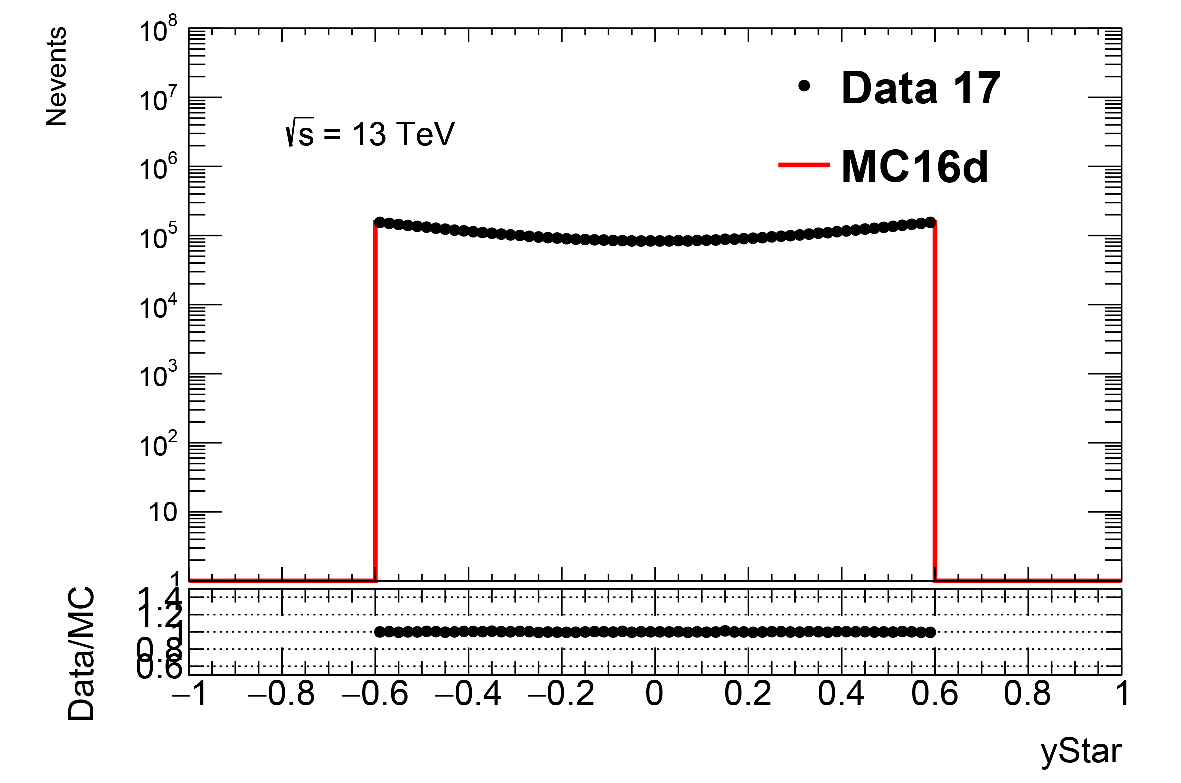
\includegraphics[width=0.45\textwidth]{fig/monitoring/1gtag/MC16d/yStar.pdf}}

 \caption{Monitoring plots for %2016 data, 
 the one-gluon selection. (a) Leading jet \pt\, %(b) $MH_T$ (missing transverse momentum calculated only from the jets in the event), 
 (b)Sub-leading jet \pt\,
 (c)) jet $\eta$,
 (d) y* between the two jets}
 \label{fig:GGmonitoring1}
\end{figure}

 \begin{figure}[htb]
 \centering
\subfloat[] {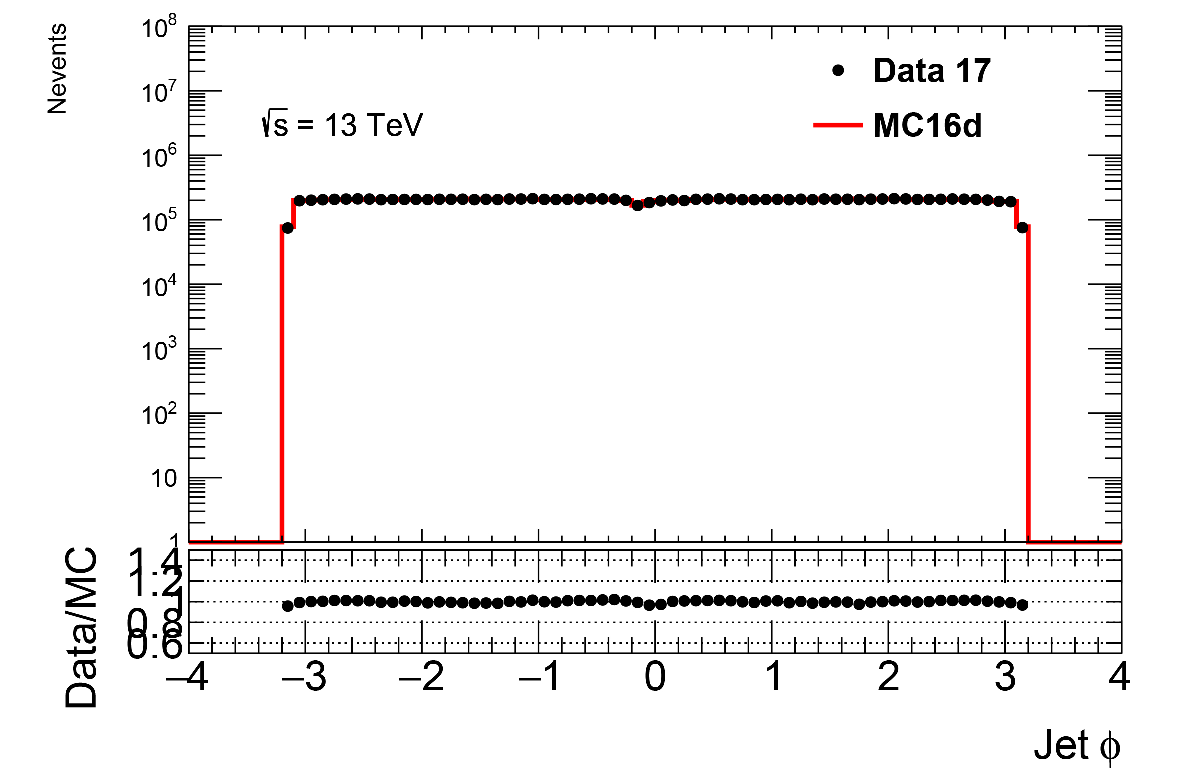
\includegraphics[width=0.45\textwidth]{fig/monitoring/1gtag/MC16d/JetPhi.pdf}}
\subfloat[] {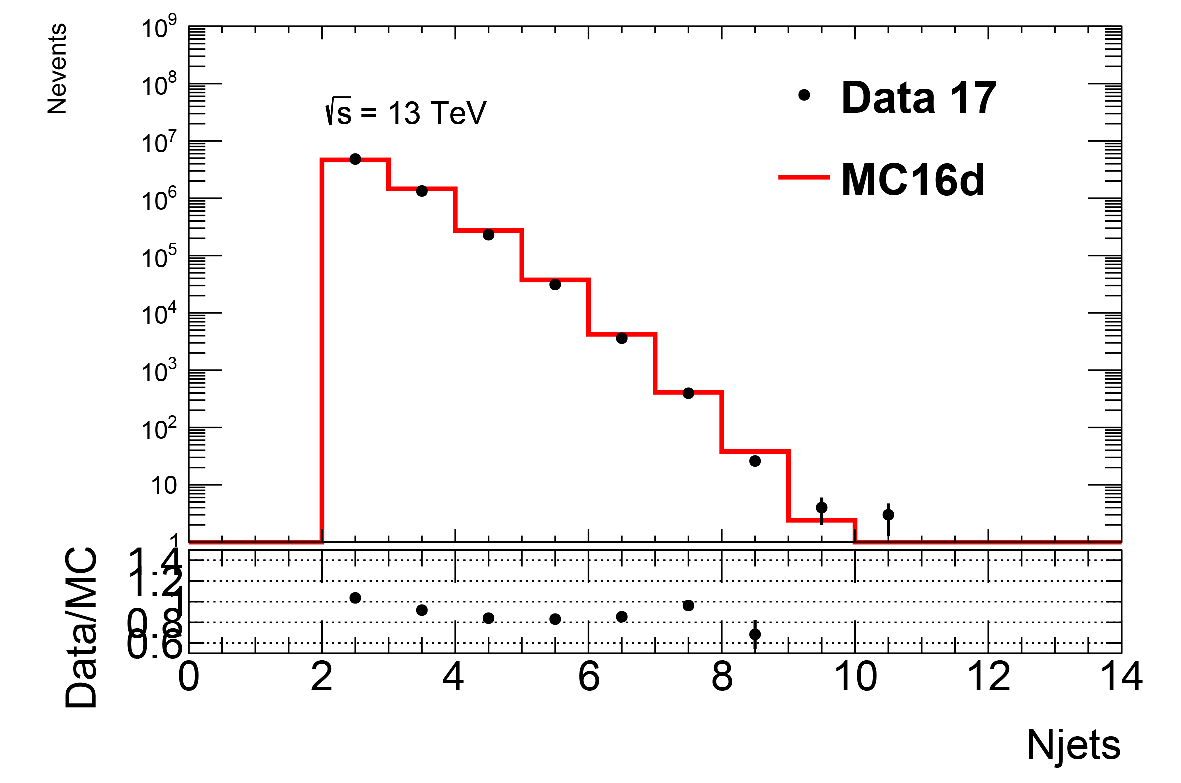
\includegraphics[width=0.45\textwidth]{fig/monitoring/1gtag/MC16d/Njets.pdf}}

 %
  \caption{Monitoring plots on the one-gluon sample. 
  (a) $\Delta\phi$ between the two jets,
  (b) number of jets.
  }
 \label{fig:GGmonitoring2}
\end{figure}


\begin{figure}[htb]
	\centering
	\subfloat[] {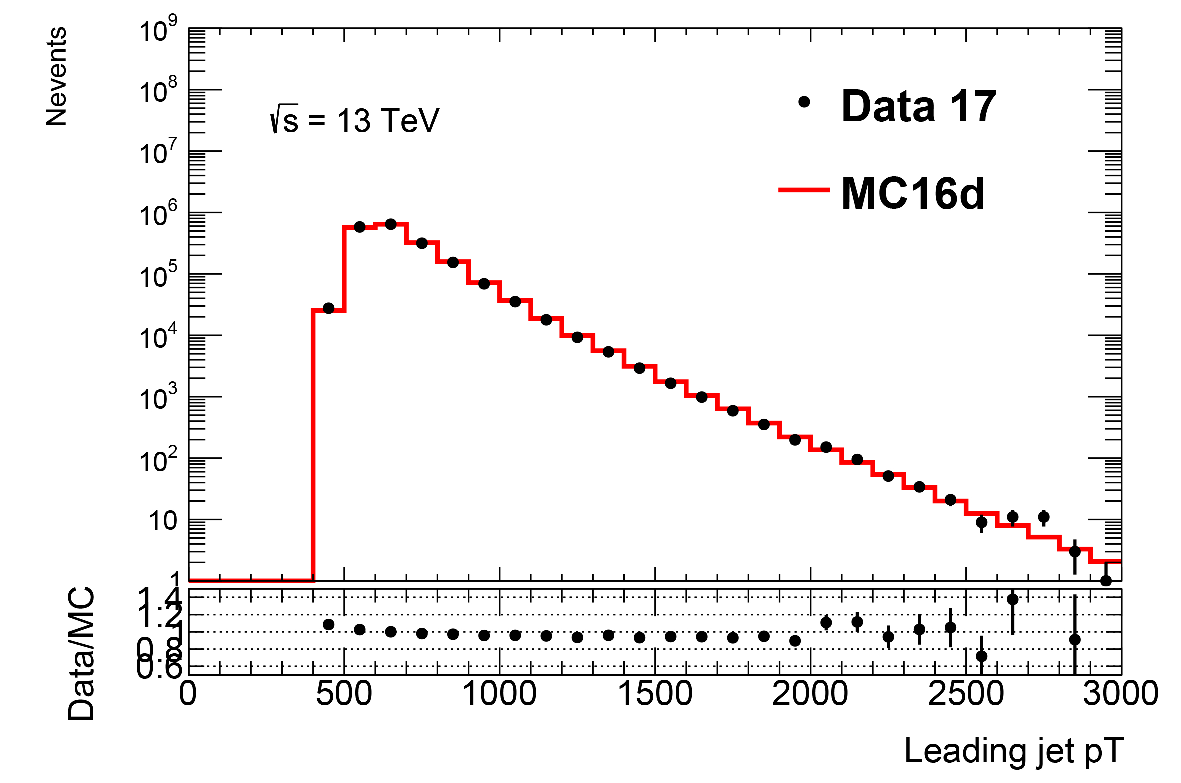
\includegraphics[width=0.45\textwidth]{fig/monitoring/2gtag/MC16d/LeadingJetPt.pdf}}
	\subfloat[] {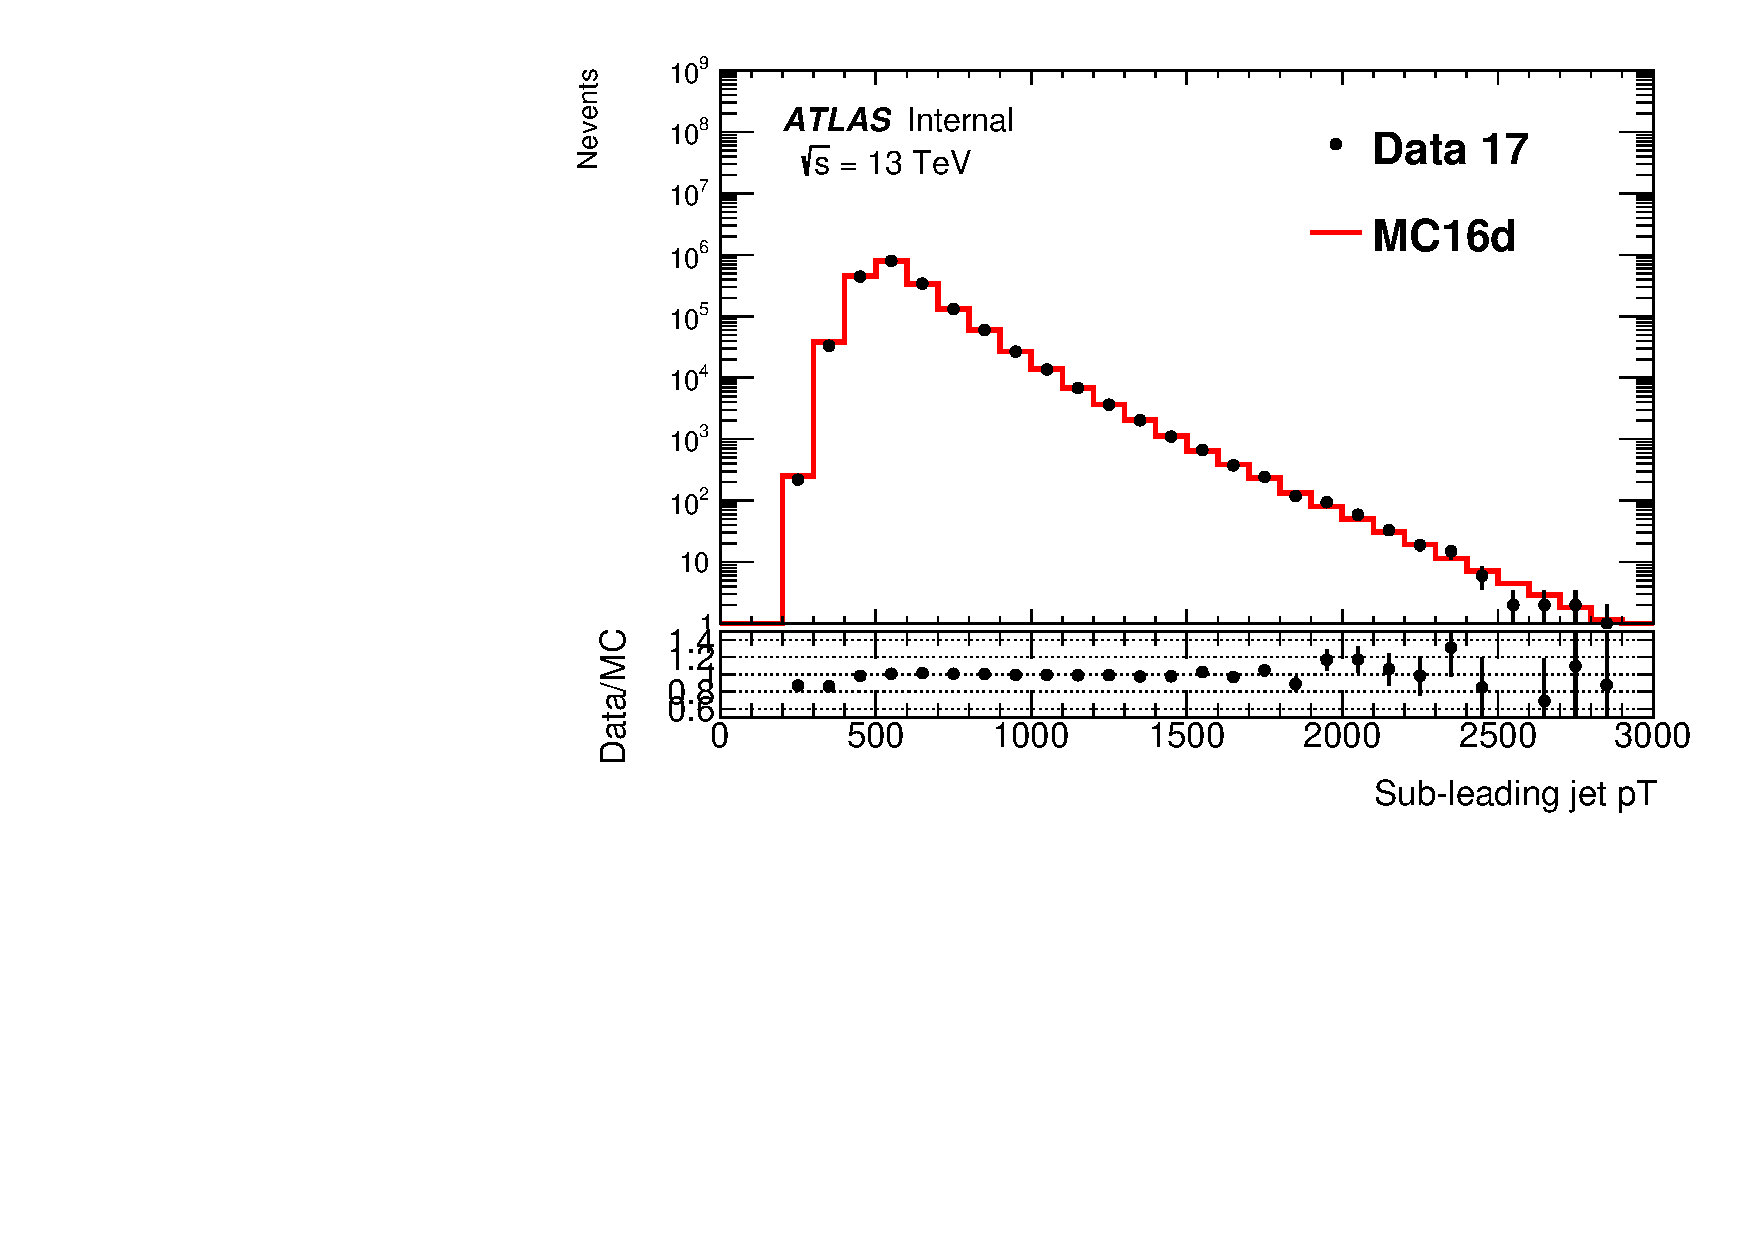
\includegraphics[width=0.45\textwidth]{fig/monitoring/2gtag/MC16d/SubLeadingJetPt.pdf}}\\
	\subfloat[] {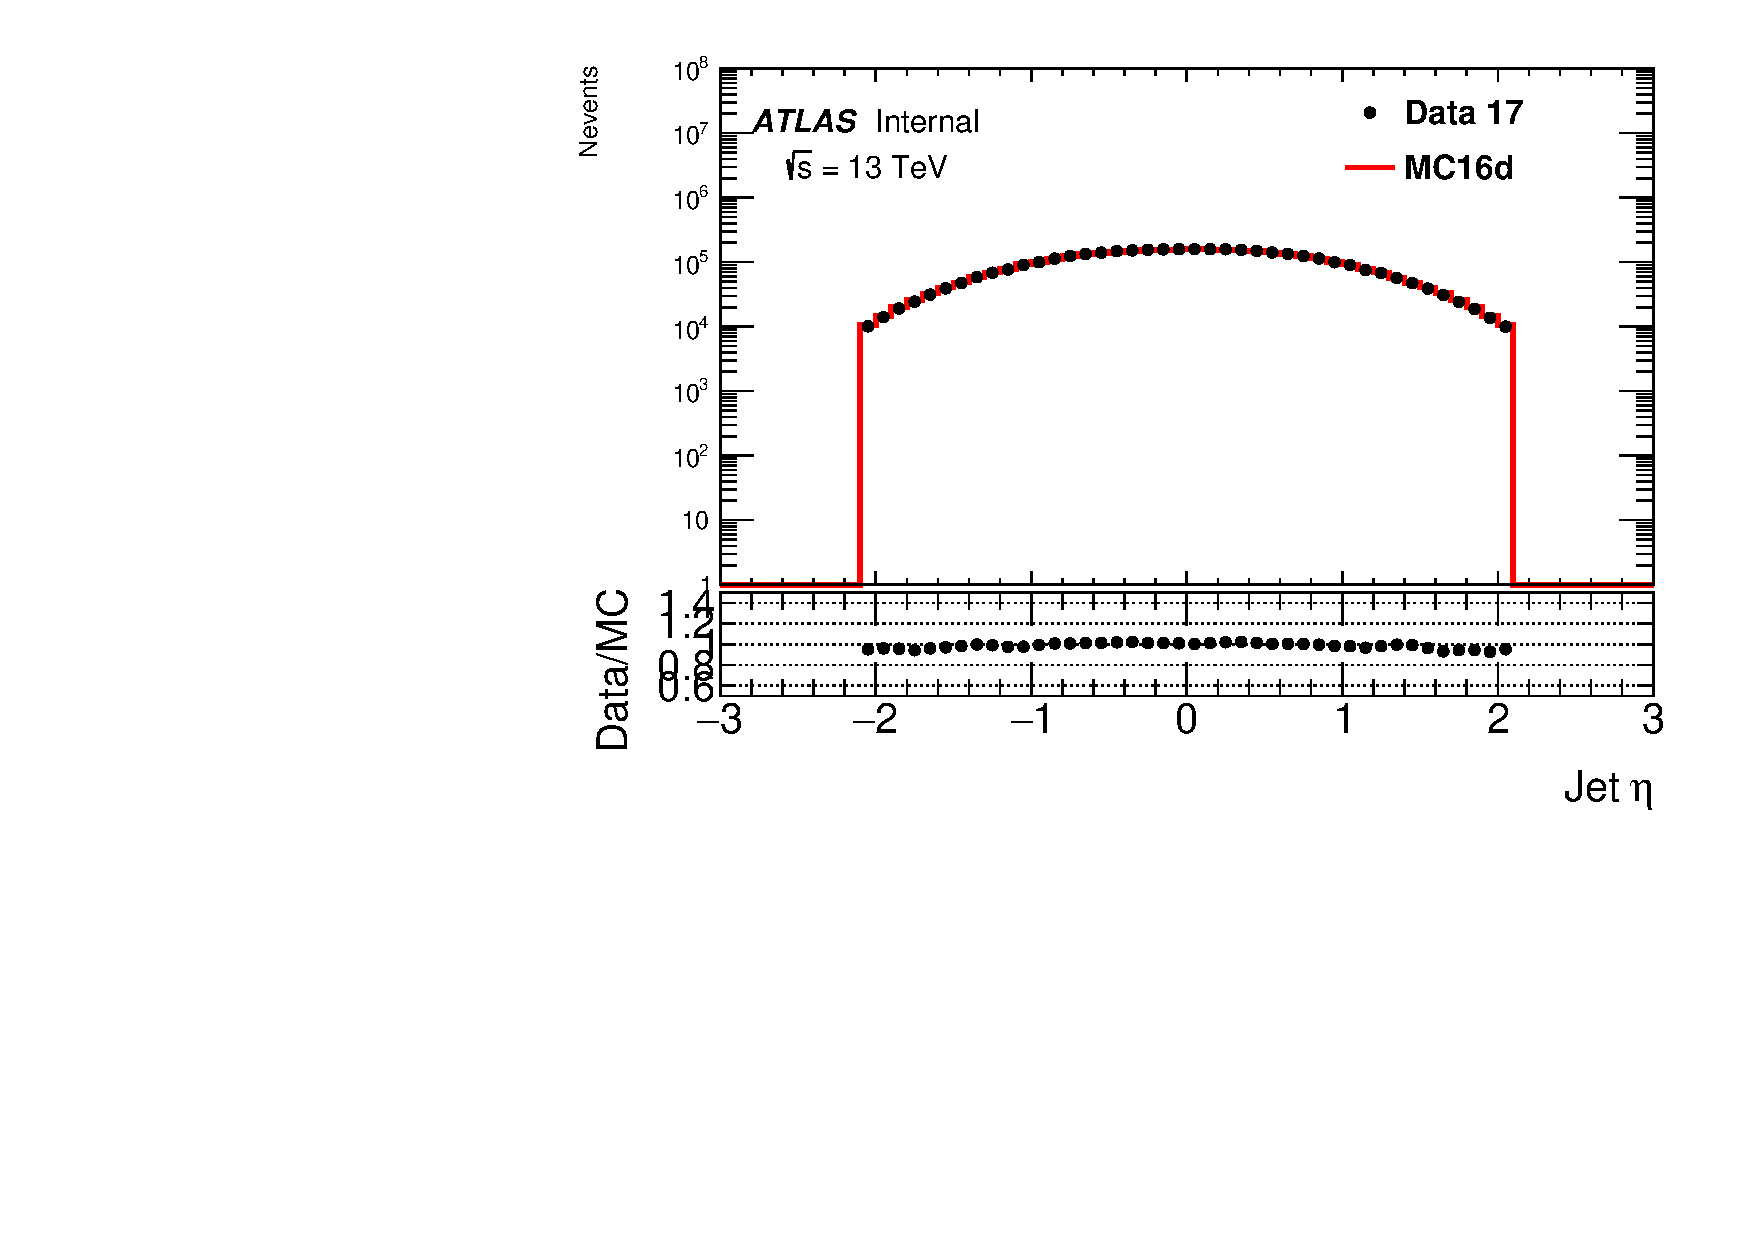
\includegraphics[width=0.45\textwidth]{fig/monitoring/2gtag/MC16d/JetEta.pdf}}
	\subfloat[] {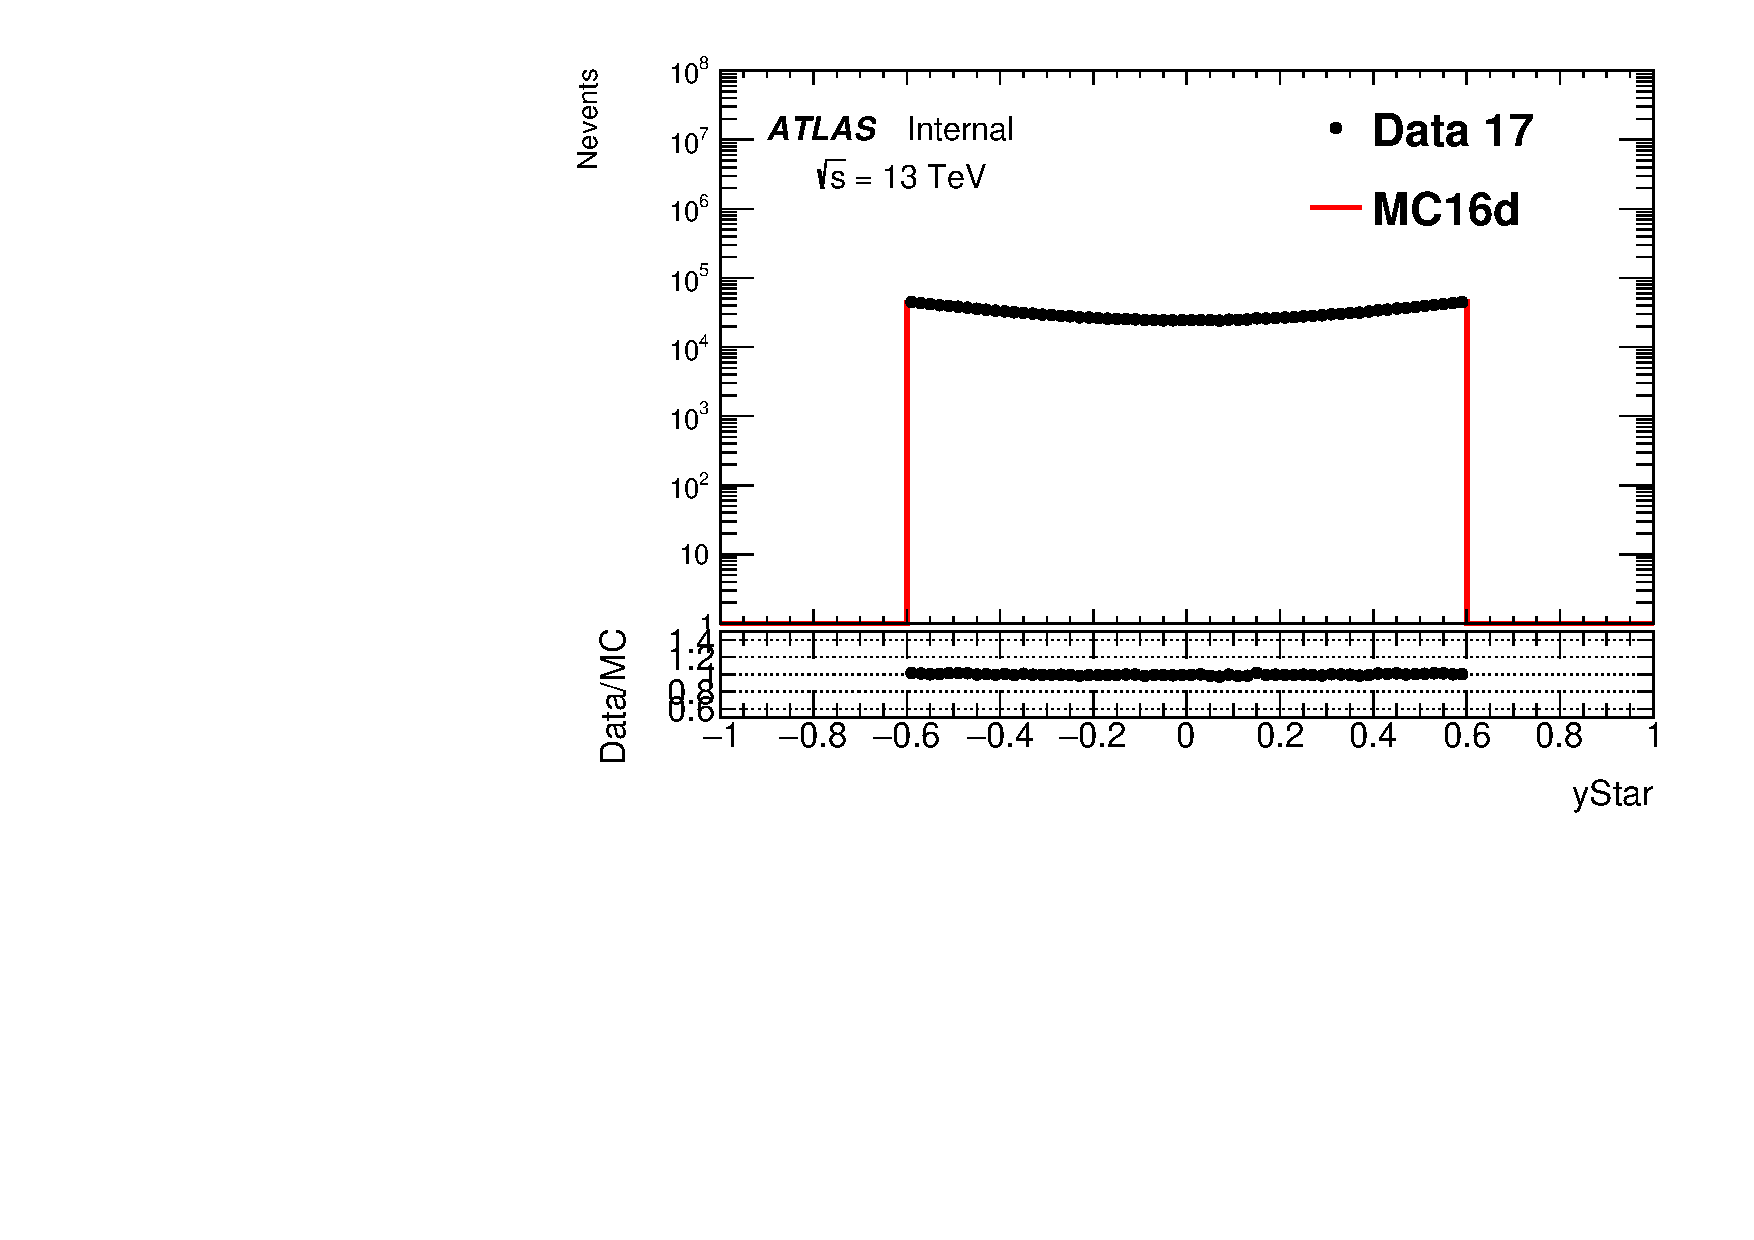
\includegraphics[width=0.45\textwidth]{fig/monitoring/2gtag/MC16d/yStar.pdf}}
	\caption{Monitoring plots for %2016 data, 
 the gluon-gluon selection. (a) Leading jet \pt\, %(b) $MH_T$ (missing transverse momentum calculated only from the jets in the event), 
(b)Sub-leading jet \pt\,
(c)) jet $\eta$,
(d) y* between the two jets}
	\label{fig:GGmonitoring3}
\end{figure}

\begin{figure}[htb]
	\centering

	\subfloat[] {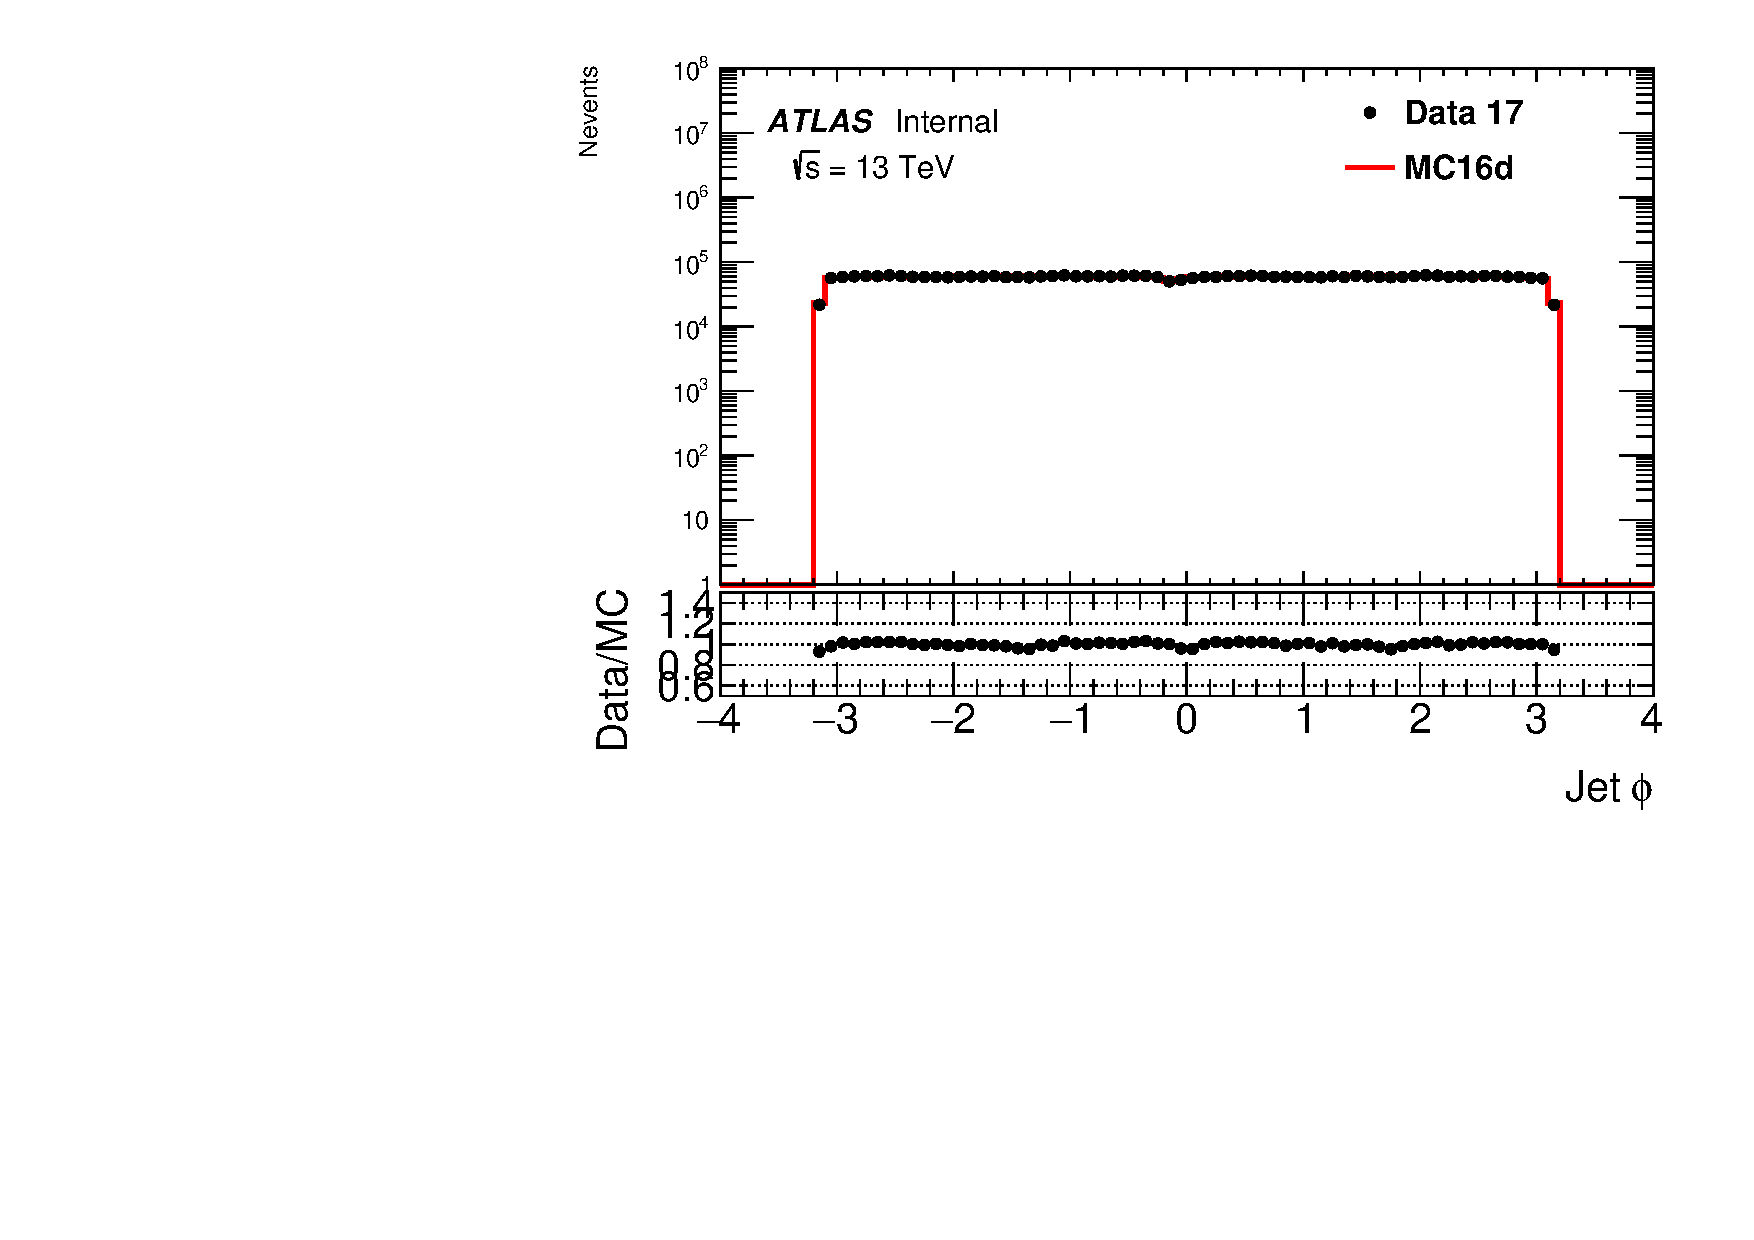
\includegraphics[width=0.45\textwidth]{fig/monitoring/2gtag/MC16d/JetPhi.pdf}}
	\subfloat[] {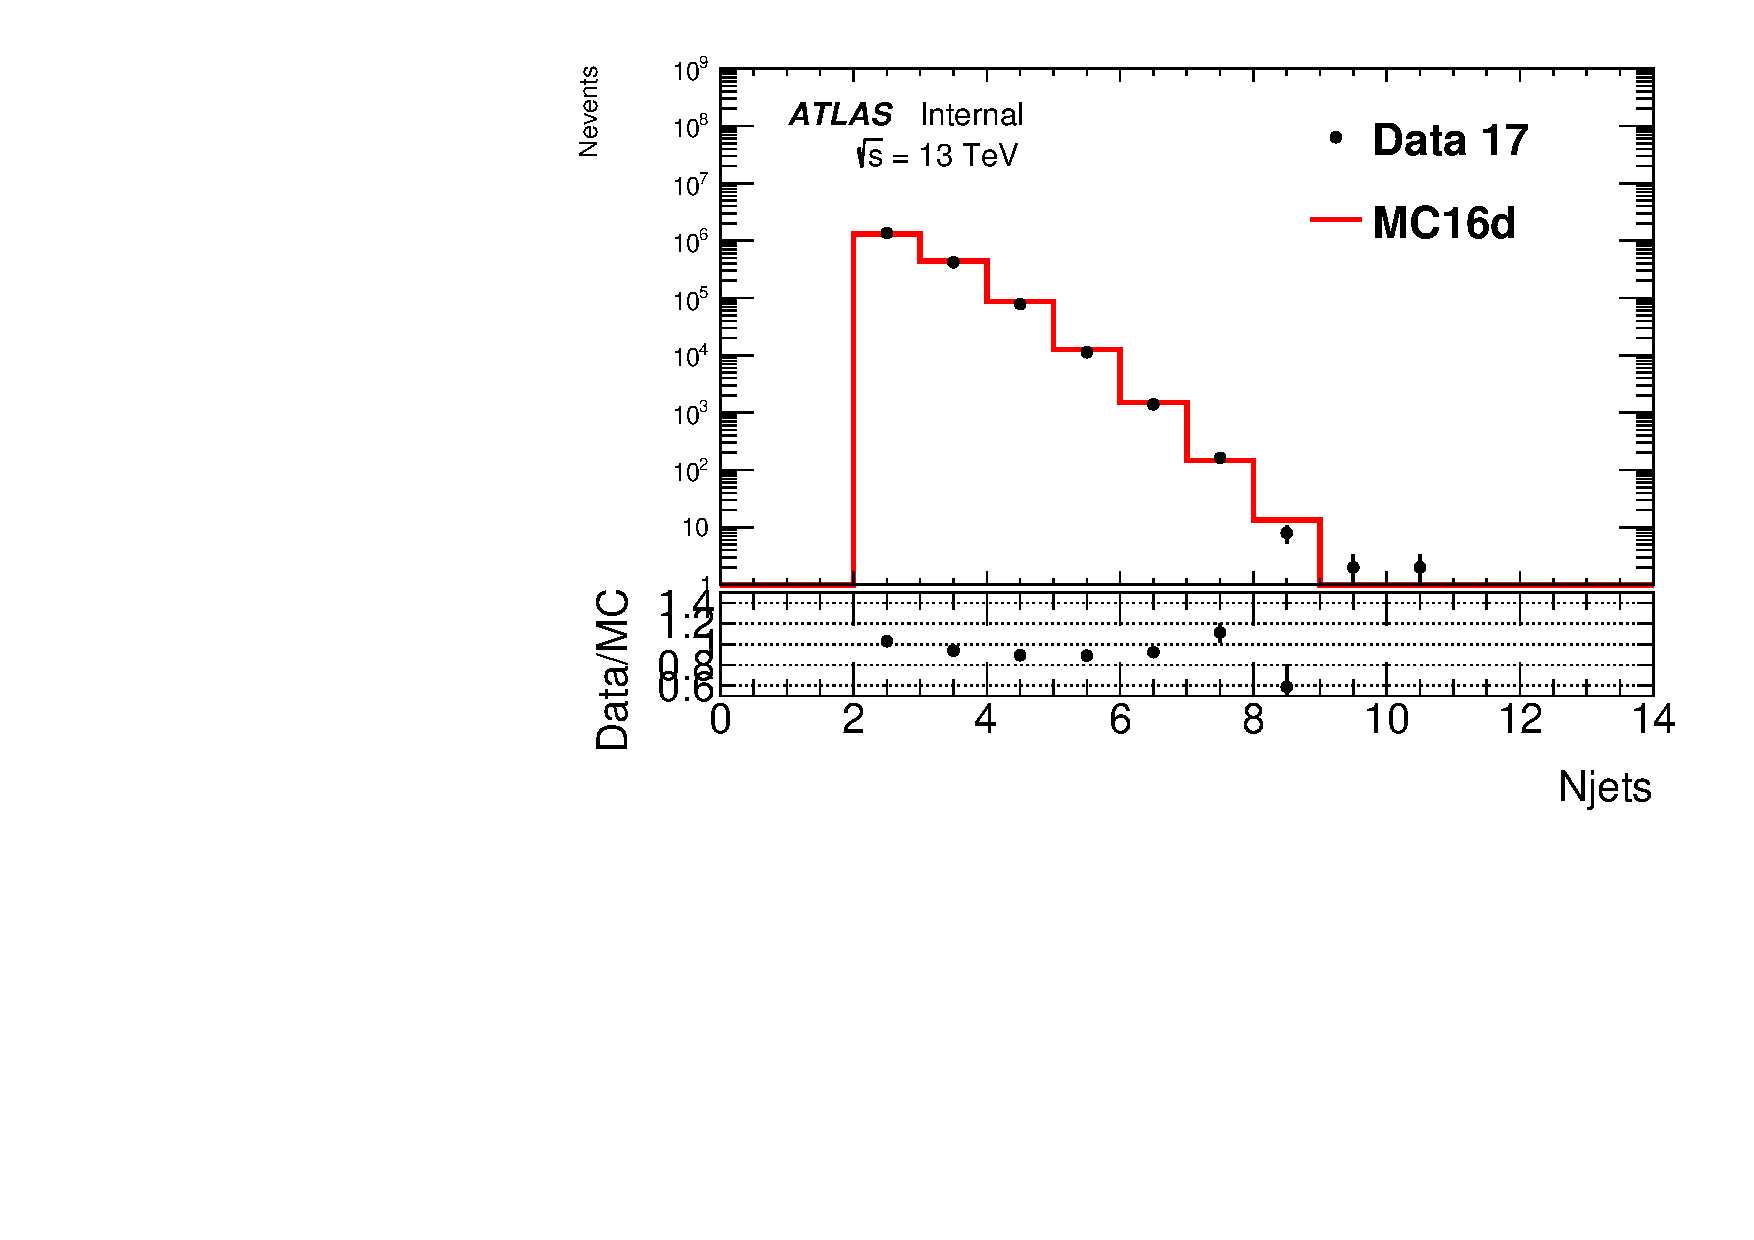
\includegraphics[width=0.45\textwidth]{fig/monitoring/2gtag/MC16d/Njets.pdf}}

  \caption{Monitoring plots on the gluon-gluon sample. 
	(a) $\Delta\phi$ between the two jets,
	(b) number of jets.
}
 \label{fig:GGmonitoring4}
\end{figure}


\clearpage

